
\documentclass{llncs}

\usepackage{amsfonts}
\usepackage{amssymb,amsmath}
\usepackage{graphicx}
\usepackage[english]{babel}
\usepackage{listings}
\usepackage{hyperref}
\usepackage[utf8]{inputenc}
\usepackage{latexsym}
\usepackage{eurosym}
\usepackage{array}
\usepackage{timestamp}
\usepackage{epstopdf}
\usepackage{multicol}
\usepackage{multirow}
\usepackage{lscape}
\usepackage{pifont}
\usepackage{stmaryrd}
\usepackage{scalerel}
\usepackage[colorinlistoftodos, textsize=tiny, shadow]{todonotes} %
\def\review{\includegraphics[width=4em]{review.jpg}}

%\usepackage[pagewise]{lineno}



%\def\thepage{\arabic{page}--[\timestamp]}
\usepackage{tikz}
\usetikzlibrary{snakes}

%\setcounter{tocdepth}{5}


% $Id: macros.tex,v 1.8 2012/07/19 22:21:36 ccamacho Exp $
% \newenvironment{definition}{\par\bf\bigskip \bigskip Definition}{\bigskip \bigskip}{\rmfamily}
% \newenvironment{example}{\par\bf\bigskip \bigskip Example}{\bigskip \bigskip}{\rmfamily}
% \newenvironment{lemma}{\par\bf\bigskip \bigskip  Lemma}{\bigskip \bigskip}{\rmfamily}
% \newenvironment{proof}{\par{\bf\bigskip \bigskip  Proof}}{\bigskip \bigskip}{\rmfamily}
% \newenvironment{proposition}{\par\bf \bigskip\bigskip  Proposition}{\bigskip \bigskip}{\rmfamily}
% \newenvironment{corollary}{\par\bf \bigskip\bigskip  Corollary}{\bigskip \bigskip}{\rmfamily}
% \newenvironment{theorem}{\par\bf \bigskip \bigskip Theorem}{\bigskip \bigskip}{\rmfamily}

%Fin de Carlos

% $Id: macros.tex,v 1.8 2012/07/19 22:21:36 ccamacho Exp $
\def\squareforqed{\hbox{\rlap{$\sqcap$}$\sqcup$}}

% Carlos
% He eliminado los cubos del qed, luego podemos mirar
% si queda algun simbolo mejor
\def\qed{
       \ifmmode\squareforqed\else{\unskip\nobreak\hfil
    \penalty50\hskip1em\null\nobreak\hfil\squareforqed
    \parfillskip=0pt\finalhyphendemerits=0\endgraf}\fi
}

%\usepackage{marginnote}
%\renewcommand{\marginfont}{\fontsize{6}{8}\selectfont}



\newcommand{\ccomens}[2]{\uwave{#1\ccomen{#2}}}
\def\lcomen#1{\footnote{\textbf{Comentario de Luis}: \textcolor{red}{#1}}}
\def\ccomen#1{\footnote{\textbf{Comentario de Carlos}: \textcolor{blue}{#1}}}
\def\acomen#1{\footnote{\textbf{Comentario de Alberto}: \textcolor{green}{#1}}}



\newcommand{\comment}[2]{\footnote{\textbf{#1}: #2}}

\newcommand{\ComaMat}{}
\newcommand{\PuntoMat}{}
%\newenvironment{proof}{Proof}


\newcommand{\ismcomment}[1]{}
\newcommand{\bdfn}{\begin{definition} \begin{rm}}
\newcommand{\edfn}{\end{rm}$ $\qed \end{definition}}

\newcommand{\bprf}{\begin{proof}}
\newcommand{\eprf}{\leavevmode\qed \end{proof}}

\newcommand{\bthm}{\begin{theorem} \begin{rm}}
\newcommand{\ethm}{\end{rm}$ $\qed \end{theorem}}

\newcommand{\bprop}{\begin{proposition} \begin{rm}}
\newcommand{\eprop}{\end{rm}$ $\qed  \end{proposition}}

\newcommand{\bcor}{\begin{corollary}\begin{rm}}
\newcommand{\ecor}{\end{rm}$ $\qed  \end{corollary}}

\newcommand{\blem}{\begin{lemma}\begin{rm}}
\newcommand{\elem}{\end{rm}$ $\qed  \end{lemma}}

\newcommand{\bfact}{\begin{fact}\begin{rm}}
\newcommand{\efact}{\end{rm}$ $\qed  \end{fact}}

\newcommand{\bex}{\begin{example}\begin{rm}}
\newcommand{\eex}{\end{rm}$ $\qed  \end{example}}

\newenvironment{defn}{\bdfn}{\edfn}
\newenvironment{proofappendix}[1]{\textbf{\emph{Proof of #1}}}{}
\newcommand{\barra}{\:| \:}
\def\y{\;\wedge\;}
\def\o{\;\vee\;}
\newcommand{\union}{\cup}
\newcommand{\contenido}{\subseteq}
\newcommand{\interseccion}{\cap}
\newcommand{\Vacio}{\emptyset}
\renewcommand{\emptyset}{\varnothing}

\newcommand{\true}{\mathtt{true}}
\newcommand{\false}{\mathtt{false}}
\newcommand{\entonces}{\mathtt{\ then\  }}
\newcommand{\sino}{\mathtt{\ else\  }}
\newcommand{\si}{\ \mathrm{if}\ }

\newcommand{\letbar}[1]{\mbox{I\kern-0.23em#1}}
\newcommand{\nat}{\letbar N}
\newcommand{\real}{\letbar R}
\newcommand{\realm}{\letbar R_+^m}
\newcommand{\Bool}{\texttt{Bool}}
%
\newcommand{\comen}[1]{
}
\newcommand{\timed}{{\mathtt{Time}}}
\newcommand{\outputs}[1]{\ensuremath{\mathtt{ outputs}(#1)}}
\newcommand{\representative}[2]{\ensuremath{\mathtt{ moreR}(#1,#2)}}
\newcommand{\msTOs}[1]{\ensuremath{\mathtt{ msTOs}(#1)}}
\newcommand{\setnttr}[2]{\ensuremath{\mathtt{ setnttr}(#1,#2)}}
\newcommand{\minTime}[1]{\ensuremath{\mathtt{ mT}(#1)}}
\newcommand{\maxTime}[1]{\ensuremath{\mathtt{ MT}(#1)}}
\newcommand{\minimo}[1]{\ensuremath{\mathtt{ min}\left\{\!#1 \!\!\!\!\right\}}}
\newcommand{\maximo}[1]{\ensuremath{\mathtt{ max}\left\{\!#1 \!\!\!\!\right\}}}
\newcommand{\FSM}{\texttt{FSM}}
\newcommand{\FSMs}{\texttt{FSMs}}
\newcommand{\EFSM}{\texttt{EFSM}}
\newcommand{\EFSMs}{\texttt{EFSMs}}
\newcommand{\TFSM}{\texttt{TFSM}}
\newcommand{\TFSMs}{\texttt{TFSMs}}
\newcommand{\TPEM}{\texttt{TPEM}}
\newcommand{\TPEMs}{\texttt{TPEMs}}

\newcommand{\SPLs}{\texttt{SPLs}}
\newcommand{\SPL}{\texttt{SPL}}
\newcommand{\PLs}{\texttt{PLs}}
\newcommand{\PL}{\texttt{PL}}
\newcommand{\FODAT}{\texttt{AT}}

\newcommand{\FODA}{\texttt{FODA}}
\newcommand{\fodaPA}{\ensuremath{\mathtt{fodaA}}}
\newcommand{\fodaPAp}{\ensuremath{\mathtt{SPLA{^\calP}}}}
\newcommand{\fodaPAbasic}{\ensuremath{\mathtt{fodaA_b}}}
\newcommand{\wellstructured}{\ensuremath{\mathtt{fodaA_{ws}}}}
\newcommand{\normalForm}{\ensuremath{\mathtt{fodaA_{nf}}}}
\newcommand{\prenormalForm}{\ensuremath{\mathtt{fodaA_{pre}}}}
\newcommand{\RSEB}{\texttt{RSEB}}
\newcommand{\PLUSS}{\texttt{PLUSS}}
\newcommand{\np}{\mathtt{np}}




 %

\newcommand{\afterCond}[1]{\texttt{afterCond}(#1)}
\newcommand{\afterInp}[1]{\texttt{afterInp}(#1)}
\newcommand{\IUT}{\texttt{IUT}}
%\newcommand{\case}{\texttt{Case :}}
\newcommand{\HOTL}{{\cal HOTL}}
\newcommand{\wc}{wild-card}

\newcommand{\calA}{{\cal A}}
\newcommand{\calB}{{\cal B}}
\newcommand{\calC}{{\cal C}}
\newcommand{\calD}{{\cal D}}
\newcommand{\calE}{{\cal E}}
\newcommand{\calF}{{\cal F}}
\newcommand{\calG}{{\cal G}}
\newcommand{\calH}{{\cal H}}
\newcommand{\calI}{{\cal I}}
\newcommand{\calL}{{\cal L}}
\newcommand{\calM}{{\cal M}}
\newcommand{\calN}{{\cal N}}
\newcommand{\calO}{{\cal O}}
\newcommand{\calP}{{\cal P}}
\newcommand{\calQ}{{\cal Q}}
\newcommand{\calR}{{\cal R}}
\newcommand{\calS}{{\cal S}}
\newcommand{\calT}{{\cal T}}
\newcommand{\calU}{{\cal U}}
\newcommand{\calV}{{\cal V}}
\newbox\arriba
\newbox\abajo
\newbox\CaracterInterno
\newbox\CaracterDerecha
\newdimen\anchura
\def\MacrosTranGeneral#1#2#3#4#5#6{%
  \setbox\CaracterInterno=\hbox{\mathsurround=0pt$\mathord#4$}
  \setbox\CaracterDerecha=\hbox{\mathsurround=0pt$\mathord#3$}
  \setbox\arriba=\hbox{$#1#2$}
  \setbox\abajo=\hbox{\mathsurround=0pt%
                      \anchura=\wd\arriba%
                      \advance \anchura by 0.5em%
                      \divide \anchura by \wd\CaracterInterno%
                      \multiply \anchura by \wd\CaracterInterno%
                      \copy\CaracterInterno\kern\SeparacionInternaFlecha
                      \hbox to \anchura{%
                          $\cleaders%
                            \hbox{\kern\SeparacionInternaFlecha\copy\CaracterInterno}
                            \hfill$}%
                      \kern\SeparacionExternaFlecha\copy\CaracterDerecha}
  \mathrel{{\buildrel\vbox{\copy\arriba \kern\SeparacionFlechaArriba} %
    \over{\copy\abajo^{#6}}}_{#5}}
  }
\def\MacrosTranGeneralProp#1#2#3#4#5{\mathchoice%
  {\MacrosTranGeneral{\scriptstyle}{#1}{#2}{#3}{#4}{#5}}
  {\MacrosTranGeneral{\scriptstyle}{#1}{#2}{#3}{#4}{#5}}
  {\MacrosTranGeneral{\scriptscriptstyle}{#1}{#2}{#3}{#4}{#5}}
  {\MacrosTranGeneral{\scriptscriptstyle}{#1}{#2}{#3}{#4}{#5}}}

\def\MacrosTran#1{%
  \def\SeparacionInternaFlecha{-0.3em}
  \def\SeparacionExternaFlecha{-0.5em}
  \def\SeparacionFlechaArriba{-3pt}
  \MacrosTranGeneralProp{#1}{\rightarrow}{-}{}{}}
\def\MacrosNoTran#1{%
  \def\SeparacionInternaFlecha{-0.3em}
  \def\SeparacionExternaFlecha{-0.5em}
  \def\SeparacionFlechaArriba{-3pt}
  \MacrosTranGeneralProp{#1\kern 0.5em}{{\not\rightarrow}}{-}{}{}}
\def\MacrosVTran#1{%
  \def\SeparacionInternaFlecha{-0.2em}
  \def\SeparacionExternaFlecha{-0.5em}
  \def\SeparacionFlechaArriba{0pt}
  \MacrosTranGeneralProp{#1}{\Rightarrow}{=}{}{}}
\def\MacrosNoVTran#1{%
  \def\SeparacionInternaFlecha{-0.2em}
  \def\SeparacionExternaFlecha{-0.5em}
  \def\SeparacionFlechaArriba{-3pt}
  \MacrosNoTranGeneralProp{#1}{\not\Rightarrow}{=}{}{}}
\def\tran#1{\ensuremath\mathbin{\MacrosTran{#1}}}
\def\vtran#1{\ensuremath\mathbin{\MacrosVTran{#1}}}
\def\notran#1{\ensuremath\mathbin{\MacrosNoTran{#1}}}
\def\novtran#1{\ensuremath\mathbin{\MacrosNoVTran{#1}}}

\newcommand{\tranp}[2]{\MacrosTran{#1}_{\!\!#2}\;}
\newcommand{\tranap}[2]{\MacrosVTran{#1}_{\!\!#2}\;}
\newcommand{\tranb}[2]{\stackrel{#1}{\Longrightarrow}_{#2}}
\newcommand{\transi}[2]{\MacrosTran{#1}_{\!\!#2}\;}
\newcommand{\SSS}{\texttt{SSadmin}}
\newcommand{\calIR}{{\cal I\!R}}
\newcommand{\calDB}{{\cal D\!B}}

\newcommand{\vtranp}[2]{\vtran{#1}_{#2}}
\newcommand{\tranop}[2]{\MacrosNoTran{#1}_{\!\!#2}\;}


\newcommand{\product}[1]{\lfloor #1\rfloor}
\newcommand{\waste}{\ensuremath{\mathtt{waste}}}
\newcommand{\ham}{\ensuremath{\mathtt{TotProb}}}
\newcommand{\nombreRegla}[1]{\ensuremath{\mathbf{[#1]}}}
\newcommand{\tvacia}{\ensuremath{\epsilon}}
\newcommand{\traces}[1]{\ensuremath{\mathtt{tr}(#1)}}
\newcommand{\products}[1]{\ensuremath{\mathtt{prod}\left(#1\right)}}
\newcommand{\nttraces}[1]{\ensuremath{\mathtt{nttr}(#1)}}


\newcommand{\straces}[1]{\ensuremath{\mathtt{SuccessfulT}(#1)}}
\newcommand{\untraces}[1]{\ensuremath{\mathtt{UnsuccessfulT}(#1)}}
\renewcommand{\prod}{\ensuremath{\mathtt{prod}}}
\newcommand{\prodp}{\ensuremath{\mathtt{prod}^\calP}}
\newcommand{\prob}[1]{\ensuremath{\mathtt{prob}\left(#1\right)}}





\renewcommand{\prod}{\ensuremath{\mathtt{prod}}}
\newcommand{\values}{\ensuremath{\mathrm{Val}}}
\newcommand{\suminputs}[1]{\ensuremath{\mathtt{sumin}(#1)}}
\newcommand{\finish}[1]{\ensuremath{\mathtt{s}(#1)}}
\newcommand{\ptraces}[1]{\ensuremath{\mathtt{ptr}(#1)}}
\newcommand{\itraces}[1]{\ensuremath{\mathtt{itr}(#1)}}
\newcommand{\completeprob}[1]{\texttt{prob}(#1)}
\newcommand{\paral}{\ensuremath{\mathbin{\wedge}}}
\newcommand{\completion}[1]{\texttt{comp}(#1)}
\newcommand{\suma}[1]{\ensuremath{\mathtt{sum}(#1)}}
\newcommand{\ctraces}[1]{\ensuremath{\mathtt{CompleteT}(#1)}}




\newcommand{\testu}[1]{\ensuremath{\mathtt{tu}(#1)}}
\newcommand{\cover}[2]{\ensuremath{\mathtt{c}_{#1}(#2)}}
\newcommand{\generateTA}[1]{\texttt{generateT}(#1)}
\newcommand{\generateTB}[1]{\texttt{generateT'}(#1)}

\newcommand{\generateTAux}[1]{\texttt{generateTAux}(#1)}
%-----------------
% feature
\newcommand{\feature}[1]{\ensuremath{\mathtt{#1}}}
\newcommand{\f}[1]{\feature{#1}}
%Optional feature
\newcommand{\ofeature}[1]{\ensuremath{\overline{\feature{#1}}}}
\newcommand{\of}[1]{\ofeature{#1}}

%trace
\newcommand{\nil}{\ensuremath{\mathtt{nil}}}
\newcommand{\exclude}[3]{\feature{#1}\mathbin{\not\Rightarrow}\feature{#2}\ \mathtt{in}\ #3}
\newcommand{\require}[3]{\feature{#1}\mathbin{\Rightarrow}\feature{#2}\ \mathtt{in}\ #3}
\newcommand{\forbid}[2]{#2\backslash\feature{#1}}
\newcommand{\mandatory}[2]{#2\Rightarrow\feature{#1}}
\newcommand{\choice}{\mathbin{\lor}}
\newcommand{\optional}[1]{\overline{#1}}
\newcommand{\trace}[1]{\ensuremath{\langle #1 \rangle}}
\newcommand{\hide}[1]{[#1]}
\newcommand{\hideA}{\hide{\calA}}

\newcommand{\aviso}[1]{{\large\textbf{\texttt{Aviso:} #1}}.}


\newcommand{\refequation}[2]{\textbf{[#1\ref{#2}]}}
\newcounter{equationi}
\newenvironment{equations}[1]{%
  \begin{list}{\fequation{#1\arabic{equationi}}}{\usecounter{equationi}}
  \def\eqitem##1{\item\label{ax:#1##1}}
}{%
  \end{list}
}
\def\sizeeq{\fontsize{8}{7}\selectfont}
\def\fequation#1{\textbf{[#1]}}
\def\refequation#1#2{\fequation{#1\ref{ax:#1#2}}}
\def\fequationas#1{\quad{\fontsize{6}{8}\selectfont\fequation{#1}}}
\def\refequationas#1#2{\quad{\fontsize{6}{8}\selectfont\refequation{#1}{#2}}}
\usepackage{tikz}
%\usepackage{tikz-uml}
\usetikzlibrary{trees,shapes,arrows,automata,positioning}
\tikzset{
            syntax/.style={
                   rectangle,
                   rounded corners,
                   draw=black, very thick,
                   minimum height=2em,
                   inner sep=2pt,
                   text centered,
                   },
            feature/.style={
             rectangle,draw
            },
            triangle/.style = {
              regular polygon,regular polygon sides=3,draw
            },
            tree/.style={
              isosceles triangle, scale=0.7, shape border rotate=90, draw
            }
        }

\def\specification{
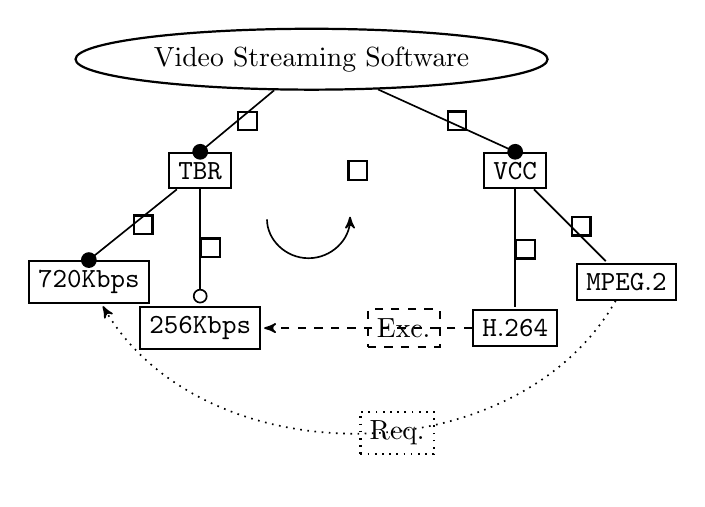
\begin{tikzpicture}[>=stealth',shorten >=1pt,auto,node distance=2cm, semithick,edge from parent]
  \node[ellipse,draw] (A)   {Video Streaming Software};
  \node[rectangle,draw]    (B) [below left  of=A]   {\TXBITRATE};
  \node[]    (AUX) [right  of=B]   {};
  \node[rectangle,draw]    (C) [right   of=AUX]   {\VCC};
  \node[rectangle,draw]    (D) [below left   of=B]   {\STZKPS};
  \node[rectangle,draw]    (E) [below of=B]   {\TFSKPS};
  \node[rectangle,draw]    (F) [below of=C]   {\HTSF};
  \node[rectangle,draw]    (G) [below right of=C]   {\MPEGTWO};

  \path (A) edge [] node {} (B.north)

            edge [] node {} (C.north)

        (B) edge [] node {} (D.north)
            edge [-o, fill] node {} (E)

        (C) edge [] node {} (F)

            edge []  node {} (G)

        (F) edge [->,dashed]  node {Exc.} (E)

        (G) edge [->,dotted,bend left=60]  node {Req.} (D)

  ;

\fill (B.north) circle (-0.1);
\fill (C.north) circle (-0.1);
\fill (D.north) circle (-0.1);
%\fill (-1.3,-1.3) circle (0.1);
%\fill (2.4,-1.3) circle (0.1);
%\fill (-3,-3) circle (0.1);

\draw [<-] (3.5,-2)  arc (360:180:15pt);

%\draw [fill=black](0,-0.35) -- (-0,-0.6) -- (0.6,-0.6)-- (0.35,-0.35)--(0,-0.35);

%\draw [<-] (A.south east)  arc (360:180:14pt);



%\draw [<-] (0.5,-0.2)  arc (360:180:14pt);

%\draw [<-] (-1.1,-4.2)  arc (360:180:14pt);

%\draw [<-] (1.5,-4.2)  arc (360:180:14pt);

%\draw [fill=black](-0.25,-4.85) -- (-0.5,-5.1) -- (0.2,-5.1)-- (0.1,-4.85)--(-0.25,-4.85);

%\draw [fill=black](2.4,-4.85) -- (2.5,-5.1) -- (3.20,-5.1)-- (2.75,-4.85)--(2.35,-4.85);

\end{tikzpicture}
}


\newcommand{\semden}[1]{\ensuremath{[\![#1]\!]}}
\newcommand{\Semden}[1]{\ensuremath{\left[\!\!\left[#1\right]\!\!\right]}}
\newcommand{\semdenp}[1]{\ensuremath{[\![#1]\!]^\calP}}
\newcommand{\Semdenp}[1]{\ensuremath{\left[\!\!\left[#1\right]\!\!\right]^\calP}}
\newcommand{\accum}{\mathtt{accum}}
\newcommand{\menos}{\mathbin{\backslash}}
\newcommand{\op}{\ensuremath{\mathtt{op}}}
\newcommand{\igecu}{\mathbin{=_{E}}}
\newcommand{\vocabulary}[1]{\ensuremath{\mathsf{voc}(#1)}}
\def\spaceFigure{0.3em}
\def\linefigure{\vspace*{\spaceFigure}\hrule\vspace*{\spaceFigure}}



\def\MPEGTWO{\feature{MPEG.2}}
\def\STZKPS{\feature{720Kbps}}
\def\HTSF{\feature{H.264}}
\def\TFSKPS{\feature{256Kbps}}
\def\TXBITRATE{\feature{TBR}}
\def\SHELL{\feature{Shell}}
\def\VCC{\feature{VCC}}
\newcommand\VSS{\feature{VSS}}

\def\oMPEGTWO{\ofeature{MPEG.2}}
\def\oSTZKPS{\ofeature{720Kbps}}
\def\oHTSF{\ofeature{H.264}}
\def\oTFSKPS{\ofeature{256Kbps}}
\def\oTXBITRATE{\ofeature{TBR}}
\def\oSHELL{\ofeature{Shell}}
\def\oVCC{\ofeature{VCC}}

\def\reduction#1{\ensuremath{\mathrm{equation}~#1}}
\newcommand{\EX}[1]{\textbf{#1}}

    \lstnewenvironment{XML}[1][]{
    \lstset{basicstyle=\fontsize{5}{6}\selectfont\ttfamily,
    linewidth=0.90\linewidth,
    %numbers=left,
    stepnumber=1,
    numbersep=10pt,
    %frame=single,
   % framerule=1.0pt,
    backgroundcolor=\color{white},
    language=HTML,
    identifierstyle=\color[rgb]{1,0,0},
    emph={schema, element, complexType, choice, simpleType, sequence, restriction, pattern}, emphstyle=\color{red},
    keywordstyle=\color[rgb]{0,0,1},
    commentstyle=\color[rgb]{0.133,0.545,0.133},
    stringstyle=\color[rgb]{0.627,0.126,0.941},
    morekeywords={xml, ref, xs, version, targetNamespace, minOccurs, maxOccurs}
    }\lstset{#1}}{}

    \lstdefinestyle{Bash}
{language=bash,
keywordstyle=\color{blue},
basicstyle=\ttfamily,
morekeywords={peter@kbpet},
alsoletter={:~$},
morekeywords=[2]{peter@kbpet:},
keywordstyle=[2]{\color{red}},
literate={\$}{{\textcolor{red}{\$}}}1
         {:}{{\textcolor{red}{:}}}1
         {~}{{\textcolor{red}{\textasciitilde}}}1,
}

%%% Local Variables:
%%% mode: latex
%%% TeX-master: "main"
%%% End:


%%%
%From macros insof...

\newcommand{\requires}{%
  \def\SeparacionInternaFlecha{-0.3em}
  \def\SeparacionExternaFlecha{-0.5em}
  \def\SeparacionFlechaArriba{-3pt}
  \ensuremath\mathbin{\MacrosTranGeneralProp{\hbox to 2em{\hss}}{\succ}{\cdot\cdot}{}{}}}


%-----------------
% feature

\newcommand{\vars}{\mathsf{vars}}
\newcommand{\maxin}{\mathsf{maxin}}
\newcommand{\logand}{\wedge}
\newcommand{\logimplies}{\mathbin{\rightarrow}}
\newcommand{\logor}{\vee}
\newcommand{\logtrue}{\top}
\newcommand{\logfalse}{\bot}
\newcommand{\logneg}{\neg}

\newcommand{\formula}{\phi}
\newcommand{\contin}{\varpropto}

\newcommand{\clausure}{\mathtt{clausure}}



\def\reduction#1{\ensuremath{\mathrm{equation}~#1}}
\newcommand{\inter}{\ensuremath{\mathsf{int}}}

\newcommand{\calFbot}{\calF_{\bot}}


\newcommand{\fA}{{\feature A}}
\newcommand{\fB}{{\feature B}}
\newcommand{\fC}{{\feature C}}
\newcommand{\fD}{{\feature D}}
\newcommand{\fE}{{\feature E}}
\newcommand{\fF}{{\feature F}}
\newcommand{\fG}{{\feature G}}
\newcommand{\fH}{{\feature H}}
\newcommand{\fI}{{\feature I}}
\newcommand{\fL}{{\feature L}}
\newcommand{\fM}{{\feature M}}
\newcommand{\fN}{{\feature N}}
\newcommand{\fO}{{\feature O}}
\newcommand{\fP}{{\feature P}}
\newcommand{\fQ}{{\feature Q}}
\newcommand{\fR}{{\feature R}}
\newcommand{\fS}{{\feature S}}
\newcommand{\fT}{{\feature T}}
\newcommand{\fU}{{\feature U}}
\newcommand{\fV}{{\feature V}}


\newcommand{\ofA}{\ofeature{A}}
\newcommand{\ofB}{\ofeature{B}}
\newcommand{\ofC}{\ofeature{C}}
\newcommand{\ofD}{\ofeature{D}}
\newcommand{\ofE}{\ofeature{E}}
\newcommand{\ofF}{\ofeature{F}}
\newcommand{\ofG}{\ofeature{G}}
\newcommand{\ofH}{\ofeature{H}}
\newcommand{\ofI}{\ofeature{I}}

% \newcommand{\lbag}{\langle}
% \newcommand{\rbag}{\rangle}

\newcommand{\natbot}{\nat_\bot}

\newcommand{\icost}{\ensuremath{\mathtt{c}}}
\newcommand{\cost}[1]{\icost(#1)}
\newcommand{\costt}[1]{\ensuremath{\mathtt{t\icost}(#1)}}
\newcommand{\costfoda}{\icost_{\fodaPA}}
\newcommand{\minc}[1]{\ensuremath{\mathtt{minc}(#1)}}

\def\novtran#1{\ensuremath\mathbin{\MacrosNoVTran{#1}}}
\def\tranold#1{\ensuremath\mathbin{\MacrosTran{#1}_{\!\!\!\!o\;}}}
\def\trannew#1{\ensuremath\mathbin{\MacrosTran{#1}_{\!\!\!\!n\;}}}

\newcommand{\productsnew}[1]{\ensuremath{\mathtt{prod}_n\left(#1\right)}}
\newcommand{\productsold}[1]{\ensuremath{\mathtt{prod}_o\left(#1\right)}}
\newcommand{\tracesnew}[1]{\ensuremath{\mathtt{tr}_n(#1)}}
\newcommand{\tracesold}[1]{\ensuremath{\mathtt{tr}_o(#1)}}

\newcommand{\runlist}{\ensuremath{\mathit{run\mbox{-}list}}}



    \newcommand*\circled[1]{\tikz[baseline=(char.base)]{
            \node[shape=circle,draw,inner sep=2pt] (char) {#1};}}

\tikzstyle{every node}=[draw=black,thick,anchor=west]
\tikzstyle{selected}=[draw=red,fill=red!30]
\tikzstyle{optional}=[dashed,fill=gray!50]
\lstset{language=Ruby,frame=trBL,basicstyle=\ttfamily\fontsize{6}{8}\selectfont}


\def\addison{Addison-Wesley}
\def\ieee{IEEE Computer Society Press}
\def\acm{ACM Press}
\def\springer{Springer}
\def\butterworths{Butterworths}
\def\elsevier{Elsevier}


\title{Probalisitic Software product lines\thanks{Research partially supported by the Spanish MINECO/FEDER project DArDOS (TIN2015-65845-C3-1-R) and the Comunidad de Madrid project SICOMORo-CM (S2013/ICE-3006).
}}
\author{Carlos Camacho \and Luis Llana\and Alberto Núñez\and Manuel Núñez}

\institute{
  Departamento Sistemas Informáticos y Computación\\
  Universidad Complutense de Madrid, Spain\\
  \email{carlos.camacho@ucm.es, llana@ucm.es, alberto.nunez@pdi.ucm.es, mn@fdi.ucm.es\\
   Draft: \timestamp
  }
}

% \author[ucm]{Carlos Camacho\corref{cor1}}
% \ead{carlos.camacho@ucm.es}


% %%%%%%%%%%%%%%%%%%%%%%%%%%%%%%%%%%%%%%%%%%%%%%%%%%%%%%%%%%%%%%%%%%%
% %%%%%%%%%%%%%%%%%%%%%%% Quitar de la versi?n final %%%%%%%%%%%%%%%%
\date{\timestamp}
\usepackage{fancyhdr}
\usepackage{timestamp}
\pagestyle{fancy}
\fancyhead{}
\fancyfoot[C]{\thepage\ --\ Draft: \timestamp}
\def\thepage{\arabic{page}--[\timestamp]}
%%%%%%%%%%%%%%%%%%%%%%% Quitar de la versi?n final %%%%%%%%%%%%%%%%
% %%%%%%%%%%%%%%%%%%%%%%%%%%%%%%%%%%%%%%%%%%%%%%%%%%%%%%%%%%%%%%%%%%%


\begin{document}
\maketitle


\begin{abstract}
We introduce a probabilistic extension of our previous
work \fodaPA: a formal framework to specify and analyze software product lines.
We use probabilistic information to identify those features that are more frequently used. This is done by computing the probability of having a feature in a specific software product line.
We redefine the syntax of \fodaPA\ to include probabilistic operators and define new operational and denotational semantics. We prove that the expected equivalence between these two semantic frameworks holds.
Our probabilistic framework is supported by a tool. We briefly comment on the characteristics of the tool and discuss the advantages of using probabilities to quantify the likelihood of having features in potential software product lines.
\end{abstract}
\textbf{Keywords;} Software Product Lines; Probabilistic Models; Formal Methods; Feature Models


%%% Local Variables:
%%% mode: latex
%%% TeX-master: "main"
%%% End:


% $Id: introduction.tex,v 1.8 2013/12/03 09:17:27 ccamacho Exp $
\section{Introduction}
\label{ref:introduction}


The main purpose of Software Product Lines (in short, \SPLs) is to produce products
while increasing productivity and shortening the time-to-market period. \SPLs\ depend
on which software products are being produced and which of them are better for
a specific criterion. When products are represented in a product line organization,
several modeling approaches can be used to increase both quality and productivity.
In most cases this is represented in the form of features, relationships and
constraints. For instance, some of these approaches are FODA~\cite{kchnp90},
RSEB~\cite{mj98} and PLUSS~\cite{k05,ebb06}.

Automatic and formal approaches arise from these graphical representations to model
variability and commonality of systems. Formal models allow for detecting errors in the early
stages of the production process. Some of the existing approaches use algebras and
semantics~\cite{szw05,kkm06,prb11,acl13}, while others use propositional or first order
logic~\cite{man02,ka07,abgf10,atfg10,nnz14}.


\begin{figure}[t]

\linefigure

\centering


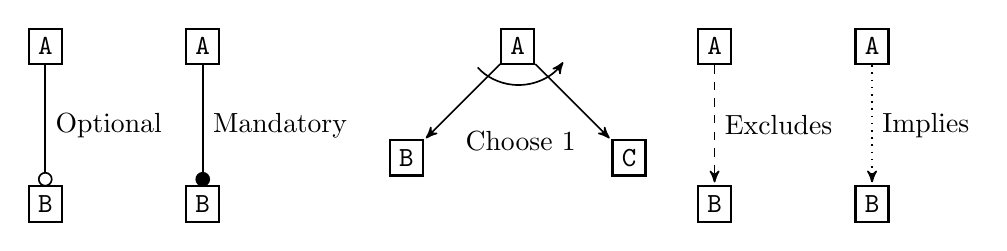
\begin{tikzpicture}[>=stealth',shorten >=1pt,auto,node distance=2cm, semithick]

  \node[rectangle,draw] (A)   {\feature{A}};
  \node[rectangle,draw] (B) [below of=A]   {\feature{B}};

  \node[rectangle,draw] (C) [right of=A]   {\feature{A}};
  \node[rectangle,draw] (D) [below of=C]   {\feature{B}};

%  \node[] (E) [right of=C]   {};
  \node[rectangle,draw,node distance=4cm] (G) [right of=C]   {\feature{A}};
  \node[rectangle,draw] (F) [below left of=G]   {\feature{B}};
%  \node[] (H) [below of=G]   {};
  \node[rectangle,draw] (I) [below right  of=G]   {\feature{C}};



  \path (A) edge [-o,shorten >=-0.05em] node[draw=none] {Optional} (B.north)
        (C) edge [-*,shorten >=-0.05em] node[draw=none] {Mandatory} (D.north)

        (G) edge [->]  node[draw=none, shift={(80:-0.5)}]{Choose 1} (F)
            edge [->]  node[draw=none] {} (I)  ;


\draw [<-] (6.8,-0.2) arc (-36:-140:20pt);

  \node[rectangle,draw,node distance=2.5cm] (J) [right of=G]   {\feature{A}};
  \node[rectangle,draw] (K) [below of=J]   {\feature{B}};

  \node[rectangle,draw] (L) [right of=J]   {\feature{A}};
  \node[rectangle,draw] (M) [below of=L]   {\feature{B}};


  \path
        (J) edge [->,dashed] node[draw=none] {Excludes} (K)
        (L) edge [->,dotted] node[draw=none] {Implies} (M)  ;

\end{tikzpicture}

\linefigure

\caption{\FODA\ Diagram representation.\label{fig:foda:relations}}

\end{figure}


% \begin{figure}[t]
% \linefigure
% \centering
% \begin{minipage}{0.2\hsize}
%         \centering
%         \EX{a}


%         \centering
%         \begin{tikzpicture}[>=stealth',shorten >=1pt,auto,node distance=1.5cm, semithick]

%           \node[rectangle,draw] (A)   {\feature{A}};
%           \node[rectangle,draw,node distance=1.1cm] (B) [below of=A]   {\feature{B}};

%           \path (A) edge [-o] node[draw=none] {} (B.north)
%           ;
%         \end{tikzpicture}

% \end{minipage}
% %
% \begin{minipage}{0.1\hsize}

%         \centering

%         \EX{b}

%         \begin{tikzpicture}[>=stealth',shorten >=1pt,auto,node distance=1.5cm, semithick]


%           \node[rectangle,draw] (C) [right of=A]   {\feature{A}};
%           \node[rectangle,draw,node distance=1.1cm] (D) [below of=C]   {\feature{B}};
%           \path (C) edge [] node[draw=none] {} (D)
%           ;
%         \fill (D.north) circle (0.1);
%         \end{tikzpicture}

% \end{minipage}
% %
% \begin{minipage}{0.33\hsize}
% \centering

%         \EX{c}

%         \begin{tikzpicture}[>=stealth',shorten >=1pt,auto,node distance=1.5cm, semithick]


%           \node[rectangle,draw] (G)    {\feature{A}};
%           \node[rectangle,draw] (F) [below left of=G]   {\feature{B}};
%           \node[rectangle,draw] (I) [below right  of=G]   {\feature{C}};

%           \path
%                 (G) edge [->]  node[draw=none] {} (F)
%                     edge [->]  node[draw=none] {} (I)

%           ;

%         \draw [<-] (0.7,-0.1) arc (360:180:14pt);

%         \end{tikzpicture}
% \end{minipage}
% \begin{minipage}{0.33\hsize}
% \centering

%         \EX{d}


%         \begin{tikzpicture}[>=stealth',shorten >=1pt,auto,node distance=1.5cm, semithick]
%           \node[rectangle,draw] (G)   {\feature{A}};

%           \node[rectangle,draw] (F) [below left of=G]   {\feature{B}};
%           \node[rectangle,draw] (I) [below right  of=G]   {\feature{C}};
%           \path
%                 (G) edge []  node[draw=none] {} (F.north)
%                     edge []  node[draw=none] {} (I.north)
%           ;
%         \fill (F.north) circle (0.1);
%         \fill (I.north) circle (0.1);
%         \end{tikzpicture}
% \end{minipage}


% \linefigure



% \begin{minipage}{0.33\hsize}
% \centering
%         \EX{e}
% \vspace*{0.3em}

%         \begin{tikzpicture}[>=stealth',shorten >=1pt,auto,node distance=1.5cm, semithick]
%           \node[rectangle,draw] (G)    {\feature{A}};
%           \node[rectangle,draw] (F) [below left of=G]   {\feature{B}};
%           \node[rectangle,draw] (I) [below right  of=G]   {\feature{C}};
%           \path
%                 (G) edge [-o]  node[draw=none] {} (F.north)
%                     edge []  node[draw=none] {} (I.north) ;
%         \fill (I.north) circle (0.1);
%         \end{tikzpicture}
% \end{minipage}
% \begin{minipage}{0.3\hsize}
%         \centering
%  \EX{f}

%         \begin{tikzpicture}[>=stealth',shorten >=1pt,auto,node distance=1.5cm, semithick]


%           \node[rectangle,draw] (A)    {\feature{A}};
%           \node[rectangle,draw] (B) [below left   of=A]   {\feature{B}};
%           \node[rectangle,draw] (C) [below right  of=A]   {\feature{C}};

%           \path
%                 (A) edge [-o]  node[draw=none] {} (B.north)
%                         edge [-o]  node[draw=none] {} (C.north)

%     (B) edge [->,dashed] node[draw=none] {} (C);
%         \end{tikzpicture}
% \end{minipage}
% \begin{minipage}{0.3\hsize}
%         \centering
%  \EX{g}

%         \begin{tikzpicture}[>=stealth',shorten >=1pt,auto,node distance=1.5cm, semithick]


%           \node[rectangle,draw] (A)    {\feature{A}};
%           \node[rectangle,draw] (B) [below left   of=A]   {\feature{B}};
%           \node[rectangle,draw] (C) [below right  of=A]   {\feature{C}};

%           \path
%                 (A) edge [-o]  node[draw=none] {} (B.north)
%                         edge [-o]  node[draw=none] {} (C.north)

%         (B) edge [->,dotted] node[draw=none] {} (C)
% ;
%         \end{tikzpicture}
% \end{minipage}
% \linefigure

% \caption{Examples of \FODA\ Diagrams.\label{section:introduction:figure:examples}}
% \end{figure}

Feature Oriented Domain Analysis~\cite{kchnp90} (in short, \FODA) is a graphical
representation of commonality and variability of systems. Figure~\ref{fig:foda:relations}
shows all \FODA\ relationships and constraints.
% and Figure~\ref{section:introduction:figure:examples}
% shows some examples of how
% \FODA\ diagrams are built.
In order to perform automatic analysis,  graphical representations
must be transformed into mathematical entities~\cite{nak10}.
Thus, it is necessary to provide the original
\FODA\ graphical representation with formal semantics base, where automated analysis can be
performed~\cite{bhst04}. This  issue is solved by using \fodaPA~\cite{acl13}, a formal
framework to represent \FODA\ diagrams using process algebras. \fodaPA\
can only be applied not only to
\FODA, but also to represent other feature-related
problems and variability models.

Costs within our formal framework refer to the required effort to add a feature to a product
under construction. This cost refers to many factors depending on the context of the
product line organization. For example, the cost of adding a feature to a product can be
equal to the number of lines of code of a software component~\cite{n07,babc09}, or the
effort, in terms of human hours, to develop that module. This effort is usually measured by using
functional metrics~\cite{j04,cg08,hko13}. The cost of adding third-party modules, both
commercial and open source, to our \SPL\ could be the time associated with integrating it into
the product line organization.

The order in which features are computed is important in many software projects and
has an  important relevance to the final cost of the project. This order can be easily incorporated
into the operational semantics of~\fodaPA. In this paper we represent costs with
natural numbers. This is not a drawback of our formalism because we can assume a
minimum cost unit, and therefore, any cost can be represented as a multiple of this unit.


\begin{itemize}
\item Hablar de las probabilidades en métodos formales.
\item Carlos debe buscar alguna referencia de SPL con probabilidades
\item Las probabilidades ayudan en los SPL. Por ejemplo en testing
  se pueden comprobar con mayor fiabilidad los productos o componentes
  que aparecen con mayor probabilidad.
\end{itemize}

El objetivo principal de éste capítulo es el de
estudiar el comportamiento de las lineas de productos
software basado en el análisis probabilístico.
Este análisis muestra cómo identificar aquella
característica mas utilizada dentro del modelo
calculando la probabilidad de encontrar
una característica dentro de una línea de productos software.

Los objetivos del presente capítulo se encuentran
clasificados de acuerdo a la siguiente estructura.
La definición de una nueva sintaxis para soportar
probabilidades basado en la sintaxis de \fodaPA.
Una nueva definición de la semántica operacional
y de la semántica denotacional que permitan
soportar probabilidades basadas en \fodaPA.
Describir las relaciones de equivalencia entre
la semántica operacional y la semántica denotacional.
Mostrar la implementación de la semántica
denotacional del modelo probabilístico determinando
la probabilidad de una característica en un modelo
de características,
sin calcular todos los productos.
Para finalizar el capítulo, se muestran los resultados
de la implementación en comparación
con los resultados obtenidos previamente en
los modelos no probabilísticos \cite{acl13,cln16}.



%%% Local Variables:
%%% mode: latex
%%% TeX-master: "main"
%%%   ispell-local-dictionary: "american"
%%% End:



% LocalWords:  formalisms

\section{$\fodaPAp$: syntax and semantics}
\label{sec:stat:sintaxMain}
In this section we introduce our language. In addition to present its syntax, we define an operational semantics and a denotational semantics. In the next section we will show the equivalence between these two semantic frameworks.


\subsection{Syntax and operational semantics}
\label{sec:stat:sintax}
Following our previous work~\cite{acl13,clc16}, we will consider a
set of features. We denote this set by $\calF$ and consider that $\feature{A}, \feature{B},
\feature{C}$ range over $\calF$. We have a special feature
$\checkmark\not\in\calF$ to mark the end  of a product. We consider a syntax similar to
\fodaPA, where probabilities are introduced both in the choice operator $P \choice_{p} Q $ and in
the optional feature operator $\ofeature{A};_{p} P$. We do not allow
\emph{degenerated} probabilities, that is, for all probability $p$ we have $0< p<1$.

The operators syntax is defined as in~\cite{acl13,clc16}.
In order to define the syntax,
we need to fix the set of \emph{features}.
From now on $\calF$ denotes a finite set  of features
and  \feature{A}, \feature{B}, \feature{C}\dots\ denote isolated features.


In this research article, like in the previous definition of SPLA~\cite{acl13,clc16},
we define and express formally that even if a feature is
represented with a mandatory relationship in the feature model,
it might not be computed in the final set or trace of valid products.
This is because of the cross tree constraints presented in the formal
representation of \fodaPA, more in specific, the \nombreRegla{excl2} and \nombreRegla{excl3} rules.
These rules, in the case of computing them, those features will be marked for hiding,
this is thanks rules \nombreRegla{hid1} and \nombreRegla{hid2} from
Figure~\ref{fig:oper-hid}, making the features
disappear in the valid products set after computing the feature model.



In the syntax of the language there are two sets of operators.
On the one hand there are \emph{main operators}, such as $\cdot\choice\cdot$, $\cdot\paral\cdot$, $\feature{A};\cdot$, $\ofeature{A};\cdot$,
$\require{A}{B}{\cdot}$, $\exclude{A}{B}{\cdot}$,
that directly correspond to relationships in \FODA\ diagrams.
On the other hand, we have \emph{auxiliary operators}, such as $\nil$, $\checkmark$, $\forbid{A}{\cdot}$, $\mandatory{A}{\cdot}$,
which we need to define the semantics of the language.


\bdfn
\label{dfn:syntax}
A \emph{probabilitistc SPL} is a term generated by the following
BNF expression:
$$
\begin{array}{ll}
P::=& \checkmark \barra \nil \barra \feature{A};P \barra
\ofeature{A};_{p} P \barra P \choice_{p} P \barra P \paral P \barra
\\
& \exclude{A}{B}{P}\barra  \require{A}{B}{P}\barra  \forbid{A}{P}\barra  \mandatory{A}{P}\\
\end{array}
$$
\noindent
where $\feature{A},\feature{B} \in \calF$ and $p\in(0,1)$. The set of terms of the
algebra will be denoted by  $\fodaPAp$.
\edfn



In order to avoid writing too many parentheses in the terms, we
assume left-associativity in binary operators and  the
following precedence in the operators (from higher to lower priority):
$\feature{A};P$, $\ofeature{A};_{p} P$, $ P \choice_{p} Q$, $P\paral Q$,
$\exclude{A}{B}{P}$, $\require{A}{B}{P}$,
$\require{A}{B}{P}$,  $\forbid{A}{P}$, and $\mandatory{A}{P}$.
In~\cite{acl13,clc16} we demonstrated that
the binary
operators are commutative and associative.
As a result, the
\emph{choose-one} operator ($\cdot\choice_{p}\cdot$) and the
\emph{conjunction} operator ($\cdot\paral\cdot$) are $n$-ary operators
instead of just binary operators.


% The Extended BNF in Definition~\ref{dfn:syntax} says
% that a term of \fodaPA\ is
% a sequence of operators and features.

There are two terminal symbols in
the language, $\nil$ and $\checkmark$,
we need them to define the semantics of the language.
%, see
%The first semantics where we will use them will be an \emph{operational} semantics.
Let us note that the products of a term in \fodaPA\ will be computed following some rules.
The computation will finish when no further steps are allowed.
This fact is represented by the $\nil$ symbol.
We will introduce rules to compute a product, with this computation
finishing when no further steps are required, a situation represented by~\nil.
During the computation of an \fodaPAp\ term,  we have
to represent the situation in which a \emph{valid product}
of the term has been computed.
This fact is represented by the $\checkmark$ symbol.

The operators $\feature{A};P$ and $\ofeature{A}_{p};P$ add the feature $\feature{A}$ to any product that can be obtained
from $P$. The operator $\feature{A};P$ indicates that $\feature{A}$ is mandatory while $\ofeature{A}_{p};P$ indicates
that $\feature{A}$ is optional and computed with probability $p$.
There are two binary operators: $P \choice_{p} Q$ and $P\paral Q$. The
first one represents a probabilistic choice. It represents a point in
the product line between two options. In this probabilistic framework,
the choice is quantified with a probability \(p\): the probability of
choosing the left hand side is \(p\) and the probability of choosing
the right hand side is \(1-p\). The operator $P\paral Q$ is the
conjunction, intuitively it combines the products of both subterms
\(P\) and \(Q\) by accumulating the features.

\begin{example}
  Let us consider the term
  $P=\feature{A};\checkmark\choice_{\frac{1}{3}}\fB;\checkmark$. This
  term will produce two products: $\{\fA\}$ with probability
  \(\frac{1}{3}\)
  and \(\{\fB\}\) with probability \(\frac{2}{3}\).
  Let us consider $Q=\fC;\ofeature{D}_{\frac{1}{5}};\checkmark$. This term will
  produce
  two products: \(\{\fC\}\) with probability \(\frac{4}{5}\) and
  \(\{\fC,\fD\}\) with probability \(\frac{1}{5}\).
  Then \(P\paral Q\) will produce the following products:
  \(\{\fA,\fC\}\) with probability \(\frac{4}{15}\),
  \(\{\fA,\fC,\fD\}\) with probability \(\frac{1}{15}\),
  \(\{\fB,\fC\}\) with probability \(\frac{8}{15}\), and
  \(\{\fA,\fC,\fD\}\) with probability \(\frac{2}{15}\).

\end{example}

The constraints are easily represented in \fodaPAp.
The operator $\require{A}{B}{P}$ represents the \emph{require}
constraint in \FODA.
The operator $\exclude{A}{B}{P}$ represents the \emph{exclusion}
constraint in \FODA.

    \bex
      The term $\require{A}{B}{\feature{A};\checkmark}$ has only one valid
      product $\{\feature{A}, \feature{B}\}$ with  probability 1.

      Let us consider
      $P=\feature{A};(\feature{B};\checkmark\choice_{\frac{1}{3}}\feature{C};\checkmark)$.
      This
      term has two valid products: The first one
      $\{\feature{A},\feature{B}\}$ with probability $\frac{1}{3}$,
      and $\{\feature{A}, \feature{C}\}$ with probability $\frac{2}{3}$.

      If we add to the previous term the following constraint
      $\exclude{A}{B}{P}$, then this new term  has only one
      $\{\feature{A},\feature{C}\}$ with  with probability
      $\frac{2}{3}$.
      This term has probability $\frac{1}{3}$ of producing nothing.
    \eex


The operator $\mandatory{A}{P}$ is necessary to define the behavior
of the $\require{A}{B}{P}$ operator:
when we compute the products of the term $\require{A}{B}{P}$, we have
to take into account whether  product  \feature{A} has been produced or not.
In the case it has been produced, we have to annotate
that we need to produce \feature{B} in the future.
The operator $\mandatory{B}{P}$  is used for this purpose.
The same happens with  the operator $\forbid{B}{P}$.
% is necessary to define the semantics of the $\exclude{A}{B}{P}$.
When we  compute the products of $\exclude{A}{B}{P}$,
if the feature \feature{A} is computed
at some point, we  annotate
that \feature{B} must not be included. The operator $\forbid{B}{P}$ indicates
that product \feature{B} is forbidden.






























%\todo{Hay que explicar los operadores probabilísticos $P \choice_{p}
%       Q$ y $\ofeature{A};_{p} P$ y la razón por la que el resto no
%       necesita probabilidades.}

%%% Local Variables:
%%% mode: latex
%%% TeX-master: "main"
%%% End:

%\subsection{Operational Semantics}
%\label{sec:stat:oper}


\begin{figure*}[h]
        \linefigure

        \centering\scalebox{0.95}{%
        $
        \begin{array}{*{3}{l@{}c@{\hspace{4em}}}}
        \nombreRegla{tick} & \checkmark\tranp{\checkmark}{1}\nil &
        \nombreRegla{feat} & \feature{A};P\tranp{\feature{A}}{1}P \\
        \nombreRegla{ofeat1} & \ofeature{A};_{p}P\tranp{\feature{A}}{p}P &
        \nombreRegla{ofeat2} & \ofeature{A};_{p}P\tranp{\checkmark}{(1-p)}\nil\\
        \nombreRegla{cho1} & \displaystyle \frac{P\tranp{\feature{A}}{p} P_1}{P\choice_{q} Q\tranp{\feature{A}}{p\cdot q} P_1}&
        \nombreRegla{cho2} & \displaystyle\frac{Q\tranp{\feature{A}}{q} Q_1}{P\choice_{p} Q\tranp{\feature{A}}{(1-p)\cdot q}Q_1}\\
        \nombreRegla{con1} & \displaystyle\frac{P\tranp{\feature{A}}{p} P_1}{P\paral Q\tranp{\feature{A}}{\frac{p}{2}}P_1\paral Q} &
        \nombreRegla{con2} & \displaystyle\frac{Q\tranp{\feature{A}}{q} Q_1}{P\paral Q\tranp{\feature{A}}{\frac{q}{2}}P\paral Q_1}\\
        \nombreRegla{con3} & \displaystyle\frac{P\tranp{\checkmark}{q}\nil, Q\tranp{\checkmark}{p}\nil}{P\paral Q\tranp{\checkmark}{p\cdot q}\nil} &\\
        \nombreRegla{con4} & \displaystyle\frac{P\tranp{\feature{A}}{p} P_1, Q\tranp{\checkmark}{q}\nil}{P\paral Q\tranp{\feature{A}}{\frac{p\cdot q}{2}} P_1} &
        \nombreRegla{con5} & \displaystyle\frac{P\tranp{\checkmark}{p}\nil,Q\tranp{\feature{A}}{q} Q_1}{P\paral Q\tranp{\feature{A}}{\frac{p\cdot q}{2}} Q_1} \\
        %
        %
        \nombreRegla{req1} & \displaystyle
        \frac{P \tranp{\feature{C}}{p} P_1,\ \feature{C}\neq\feature{A}}{\require{A}{B}{P}
                \tranp{\feature{C}}{p} \require{A}{B}{P_1}} &
        \nombreRegla{req2} &  \displaystyle
        \frac{P \tranp{\feature{A}}{p} P_1}{\require{A}{B}{P}\tranp{\feature{A}}{p} \mandatory{B}{P_1}} & \\
        % \nombreRegla{req3} & \displaystyle
        % \frac{P \tranp{\feature{B}}{p} P_1}{\require{A}{B}{P}
        %   \tranp{\feature{B}}{p} P_1} &
        \nombreRegla{req3} &  \displaystyle
        \frac{P \tranp{\feature{\checkmark}}{p} \nil}{\require{A}{B}{P}
                \tranp{\feature{\checkmark}}{p} \nil}\\
        \nombreRegla{excl1} &    \displaystyle
        \frac{P \tranp{\feature{C}}{p} P_1,\ \feature{C}\neq\feature{A},\  \feature{C}\neq\feature{B}}{
                \exclude{A}{B}{P}\tranp{\feature{C}}{p} \exclude{A}{B}{P_1}} &
        \nombreRegla{excl2} & \displaystyle
        \frac{P \tranp{\feature{A}}{p} P_1}{\exclude{A}{B}{P}
                \tranp{\feature{A}}{p}\forbid{B}{P_1}} \\
        \nombreRegla{excl3} & \displaystyle
        \frac{P \tranp{\feature{B}}{p} P_1}{\exclude{A}{B}{P}\tranp{\feature{B}}{p}\forbid{A}{P_1}}
        &
        \nombreRegla{excl4} & \displaystyle
        \frac{P \tranp{\checkmark}{p} \nil}{\exclude{A}{B}{P}\tranp{\checkmark}{p}\nil}\\

        \nombreRegla{forb1} & \displaystyle
        \frac{P \tranp{\feature{B}}{p} P_1,\ \feature{B}\neq\feature{A}}{\forbid{A}{P}
                \tranp{\feature{B}}{p} \forbid{A}{P_1}} &
        \nombreRegla{forb2} & \displaystyle
        \frac{P \tranp{\checkmark}{p} \nil}{\forbid{A}{P}
                \tranp{\checkmark}{p} \nil}  \\
        %      \nombreRegla{forb3} & \displaystyle
        %     \frac{P\tran{\feature{A}}P_2 \tran{\feature{F}} P_1}{\forbid{A}{P}
        %       \tran{\feature{B}} \forbid{A}{P_1}},\ \feature{B}\neq\feature{A} &
        %      \nombreRegla{forb4} & \displaystyle
        %     \frac{P\tran{\feature{A}}P_2 \tran{\feature{\checkmark}} P_1}{\forbid{A}{P}
        %       \tran{\checkmark} \nil}\\
        %
        %
        %
        \nombreRegla{mand1} &  \displaystyle\frac{P\tranp{\checkmark}{p} \nil}{\mandatory{A}{P}
                \tranp{\feature{A}}{p} \checkmark}  &
        \nombreRegla{mand2} &  \displaystyle\frac{P\tranp{\feature{A}}p P_1}{\mandatory{A}{P}\tranp{\feature{A}}p P_1} \\
        \nombreRegla{mand3} &  \displaystyle\frac{P\tranp{\feature{B}}p
                P_1,\ \feature{A}\neq\feature{B}}{\mandatory{A}{P}\tranp{\feature{B}}p \mandatory{A}{P_1}}
        \\
        \multicolumn{4}{c}{\feature{A},\feature{B},\feature{C}\in\calF,\ a\in\calF\cup\{\checkmark\}}

        \end{array}
        $}

        \noindent

        \linefigure

        \caption{\fodaPAp\ operational semantics.  \label{fig:sos-rules}}


\end{figure*}

In Figure~\ref{fig:sos-rules} we present the set of rules formally defining  the operational behavior of
\fodaPAp. These rules essentially coincide with the ones corresponding
\fodaPA~\cite{acl13}, but with the addition of probabilities. Next we focus 
on the explanation of the role of probabilities. Rules
$\nombreRegla{tick}$ and $\nombreRegla{feat}$
show the corresponding feature with probability 1.
%
Rules  $\nombreRegla{ofeat1}$ and $\nombreRegla{ofeat2}$ deal with the
probabilistic optional feature. The feature can be chosen with probability
$p$ and can be rejected with probability  $1-p$. Let us note that both probabilities
are not null.
%
Rules $\nombreRegla{cho1}$ and $\nombreRegla{cho2}$ define the
behavior of the probabilistic choice operator. The left branch is
selected with probability $p$ and the right with probability $1-p$.
%
It is important to note rules for the conjunction operator
(Rules $\nombreRegla{con1}$ to $\nombreRegla{con4}$)
distribute the probability equitably between both
branches, that is, $\frac{1}{2}$.
%
Rule $\nombreRegla{con5}$ requires that both branches agree on the
termination of a product.
%

\blem\label{lem:check}
  Dados los términos $P,Q\in\fodaPA$ y la probabilidad $p\in(0,1]$, $P\tranp{\checkmark}{p}{Q}$ si y sólo si $Q=\nil$.
\elem


\begin{itemize}
\item Hay que introducir la notatición de multiconjuntos
\item Hay que explicar la necesidad de los multiconjuntos.
\item $\ham(P)$ es lo que suman las probabilidades de los productos
  del término.
\end{itemize}

\bdfn\label{def:trtrantions}
\begin{enumerate}
\item $P\vtranp{s}{p}Q$ iff si $s=a_1a_2\cdots a_n$ y $p=p_1\cdot
  p_2\cdot \cdots p_{n}$ and
  \begin{displaymath}
    P=P_0\tranp{a_1}{p_1}P_1\tranp{a_2}{p_2}P_2\cdots P_{n-1}\tranp{a_n}{p_n} P_n=Q
  \end{displaymath}
\item
  $(pr,p)\in\prodp(P)$ si y sólo si $p>0$ y $p=\sum\lbag q\ |\
  P\vtranp{s\checkmark}{q} Q \y \product{s}=pr \rbag$
\item $\ham(P)=\rbag p\ |\ \exists pr: (pr,p)\in\prodp(P)$
\item $\waste(P) = 1-\ham(P)$
\end{enumerate}

\edfn


\begin{itemize}
\item Si tengo una traza su probabilidad es mayor que 0.
\item La suma de las probabilidades de todos los productos están en el
  intervalo [0,1].
\end{itemize}



\blem\label{lem:sum:prob}
  Let  $P,\ Q\in\fodaPAp$,
  \begin{enumerate}
  \item $P\tranp{\feature{A}}{p}Q$ then $p\in(0,1]$.
  \item $P\vtranp{s}{p}Q$ then $p\in(0,1]$.
  \item
    $\sum \lbag p\, |\ \exists \feature{A}\in\calF,\ Q\in\fodaPA:\
    P\tranp{\feature{A}}{p}Q \rbag\in[0,1]$

  \item
    $\sum \lbag p\, |\ \exists \feature{s}\in\calF^*,\ Q\in\fodaPA:\
    P\tranp{\feature{s}}{p}Q \rbag\in[0,1]$
  \item
    $\ham(P)\in [0,1]$
  \end{enumerate}
\elem





%%% Local Variables:
%%% mode: latex
%%% TeX-master: "main"
%%% End:

\section{Consistencia del modelo probabilístico}

La consistencia del modelo probabilístico se basa en la
consistencia del modelo no probabilístico. Esto implica
que deberá ser definida una función que permita realizar
una traducción directa entre \fodaPAp y \fodaPA,
de esta manera se demostrará que esta particularización
del modelo es consistente si y sólo si el modelo
no probabilístico lo es.

%\begin{itemize}
%\item Define the non probabilistic model.
%\item Define a function that remove probabilities.
%\item The probabilistic model has the same products a the corresponding non probabilistic one
%\item The probabilistic model is consistent iff corresponding non probabilistic one is consistent
%\end{itemize}

La sintaxis del modelo no probabilístico es presentada en la definición \ref{dfn:syntax}
%\bdfn
%A \emph{non-probabilistic software product line} is a term generated by the following Extended BNF-like expression:
%$$
%\begin{array}{ll}
%  P::=& \checkmark \barra \nil \barra \feature{A};P \barra
%    \ofeature{A};_{p} P \barra P \choice_{p} Q \barra P \paral Q \barra
%  \\ 
%  & \exclude{A}{B}{P}\barra  \require{A}{B}{P}\barra  \forbid{A}{P}\barra  \mandatory{A}{P}\\ 
%\end{array}     
%$$
%\noindent 
%where $\feature{A} \in \calF$. We will denote the set of terms of this algebra by $\fodaPA$.
%\edfn

\bdfn
  Se define la función $\np:\fodaPAp\mapsto \fodaPA$, 
  eliminando las información relacionada a las probabilidades.
  \begin{displaymath}
     \np(P)=
     \begin{cases}
       \ofeature{A};P & \mathrm{si}\ P=\feature{A};_pP\\
       P \choice Q & \mathrm{si}\ P \choice_{p} Q \\
       P & \mathrm{en\ cualquier\ otro\ caso}
     \end{cases}
  \end{displaymath}
\edfn



\bprop\label{prop:relnonprob}
  Dados los términos $P,Q\in\fodaPAp$, 
  
  \begin{enumerate}
  \item\label{prop:relnonprob-a} $P\vtranp{s}{p}Q$ si y sólo si $\np(P)\vtran{s}\np(Q)$.
  \item\label{prop:relnonprob-b} $pr\in\prod(\np(P))$ si y sólo si existe $p>0$ tal que $(pr,p)\in\prodp(P)$.
  \item\label{prop:relnonprob-c} $pr\in\semden{\np(P)}$ si y sólo si existe $p>0$ tal que $(pr,p)\in\semdenp{P}$.
  \item\label{prop:relnonprob-d} Existe $p\in(0,1)$ tal que $(pr,p)\in\prodp(P)$ si y sólo si existe $q\in(0,1)$ tal que $(pr,q)\in\semdenp{P}$.
  \end{enumerate}
  
  
  
  \begin{proof}
    La demostración de las secciones ~\ref{prop:relnonprob-a} y~\ref{prop:relnonprob-c} de la proposición 
    \ref{prop:relnonprob} es trivial ya que las reglas consideradas en ~\cite{acl13}
    son las mismas que las presentadas en el modelo probabilístico, simplemente
    eliminando la información relacionada a las probabilidades. La sección ~\ref{prop:relnonprob-b} 
    de la proposición \ref{prop:relnonprob} es una consecuencia directa de la sección ~\ref{prop:relnonprob-a}
    de la proposición \ref{prop:relnonprob}. 
\todo{Hay que escribir esta demostración más detallada}
  \end{proof}
\eprop

% As a direct consequence of the previous result we have the following Corollary.
% \bcor\label{cor:relnonprob}
%   Let $P,Q\in\fodaPAp$, There exists $p\in(0,1)$ such that
%   $(pr,p)\in\prodp(P)$ iff there exist $q\in(0,1)$ such that
%   $(pr,q)\in\semdenp(P)$.  
% \ecor

%%% Local Variables: 
%%% mode: latex
%%% TeX-master: "../../main"
%%% ispell-local-dictionary: "castellano"
%%% End: 

\subsection{Denotational Semantics}
\label{sec:stat:den}
\mncomment{Comprobad que he interpretado bien lo que ponia en los itemizes originales}

Next we define a denotational semantics for the terms of our language. The main features of the semantic domain are that we consider products (set of features) with probability,
each product appears one and the sum of all the probabilities
associated with products belongs to the interval $(0,1]$. First, we
precisely define the members of the semantic domain. 

%\todo{Explicar el modelo con más detalle,  y el motivo por el que se necesitan multiconjnutos}

\mncomment{Me he bloqueado. Se quiere definir primero el dominio
  semantico, supongo. Asi que habria que definir $\calM$, creo. Luego,
  durante el resto de la seccion, en lugar de decir $M \subseteq
  \calP(\calF)\times [0,1]$ habria que decir $M\in \calM$, no? Supongo
  esto y continuo. Si he supuesto algo mal, corregidlo,
  please.}\lcomen{Ha veces que lo que hay son elementos 
$MM \subseteq \calP(\calF)\times [0,1]$ que no cumplen la condición de \calM.}

\bdfn\label{def:den:pr}
We define the semantic domain $\calM$ as the largest set $\calM\subseteq\calP(\calP(\calF)\times
  (0,1]))$ such that if $M\in\calM$ then the following
  conditions hold:
  \begin{itemize}
  \item If $(P,q)\in M$ and $(P,r)\in M$ then $q=r$.
  \item $0\leq \sum \lbag q \ | \ \exists P: (P,q)\in M\rbag \leq 1$.
  \end{itemize}
%\edfn

%\begin{itemize}
%\item The multisets in will appear in the operational semantics.
%\item We need to convert these multisets into sets of the model. It is
%  possible if the conditions of Proposition~\ref{prop:pr:accum} hold.
%\end{itemize}

%\bdfn
Let $M$ a multiset  with elements in the set $\calP(\calF)\times [0,1]$.
We define the operator $\accum$ as follows:
  $$\accum(M) = \left\{(P,p)\ \left| \ p=\sum_{(P,q)\in M}q \wedge p>0\right. \right\}$$
\edfn

The following result is immediate.
\bprop\label{prop:pr:accum}
 Let $M$ be a multiset with elements in the set $\calP(\calF)\times
 [0,1]$
 \mncomment{otra vez lo de multiset. Puede que yo no haya entendido
   algo? Pero vamos, si es un multiset, no tiene sentido que ponga
   $M\subseteq \calP(\calF) \times [0,1]$.}\lcomen{En la mayoría de
   los operadores semántics salen multiconjuntos. Por eso $M$ debe ser
 un multiconjunto.}
 %be a multiset, 
 If $1\geq\sum\lbag q\ |\ (P,q)\in M\rbag$
 then $\accum(M)\in\calM$.
\eprop


Next we define the operators of the denotational semantics. Multisets
meeting the conditions of the previous Proposition appear when
defining these operators. For instance, the prefix operator
$\semden{\fA;}(M)$ should add feature $\fA$ to any product in $M$. Let
suppose that 
$M=\{
   (\{\fB,\fA\},\frac{1}{2}), 
   (\{\fB\},\frac{1}{2})\}$. 
If we add $\fA$ to the products of $M$, we obtain the product
$\{\fA,\fB\}$ repeated twice with probability $\frac{1}{2}$. So we
need to apply the function $\accum$ to accumulate both probabilities
and obtain a single product with probability $1$. Also in this
definition we use the multiset union denoted by $\uplus$.


\bdfn\label{def:semantic:operators}
  Let $M,M_1,M_2\in\calM$, $\fA,\fB\in\calF$, and $p\in(0,1]$. For any operator appearing in
  Definition~\ref{sec:stat:sintax} we define its denotational operator
  as follows:
  \begin{itemize}

  \item $\semdenp{\nil}=\emptyset$

  \item $\semdenp{\checkmark}=\{(\emptyset,1)\}$

  \item
    $\semdenp{\feature{A};\cdot}(M)=
      \accum\bigl(\lbag(\{\feature{A}\}\cup P,p)\ |\ (P,p)\in M\rbag\bigr)
      % \accum\bigl(
      %    \{ (\{\feature{A}\} \cup P,p ) |\   (P,p) \in M\}\bigr)
         $

  \item
    $\semdenp{\ofeature{A};_{r}\cdot}(M)=
                \accum\bigl(\lbag(\emptyset , 1-r )\rbag\uplus\lbag (\{\feature{A}\}\cup P, r\cdot p ) \ |\ (P,p) \in M\rbag\bigr)$

  \item
    $\semdenp{\cdot\choice_{r}\cdot}(M_{1},M_{2})=\accum\bigl(\lbag(P,r\cdot p  ) \ |\ (P,p) \in
    M_{1}\rbag \uplus \lbag(Q, (1-r)\cdot q  ) \ |\ (Q,q) \in M_{2}\rbag\bigr) $
  \item
    $
        \semdenp{\cdot\paral\cdot}(M_{1},M_{2})= \accum\Bigl(
                \lbag (P\cup Q, p\cdot q)  |\ (P,p) \in M_{1},\ (Q,q) \in M_{2}\rbag\Bigr)
    $

  \item
    $\semdenp{\require{A}{B}{\cdot}}(M)=\accum\left(\begin{array}{l}
      \lbag\bigl(P,p\bigr)\ |\  (P,p)\in M, \feature{A}\not\in P\rbag\ \uplus\\
      \lbag\bigl(\{\feature{B}\}\cup P ,p\bigr)\ |\ (P,p)\in M, \feature{A}\in P\rbag \\
      \end{array}\right)$

  \item
    $\semdenp{\exclude{A}{B}{\cdot}}(M)=\begin{array}[t]{l}
      \{(P,p)\ |\ (P,p)\in M, \feature{A}\not\in P\}\cup\\
      \{(P,p)\ |\ (P,p)\in M, \feature{B}\not\in P\}
      \end{array}$

    \item $\semdenp{\mandatory{A}{\cdot}}(M) = \semdenp{\feature{A};{\cdot}}(M)$

    \item
      $\semdenp{\forbid{A}{\cdot}}(M) = \{(P,p)\ |\ (P, p) \in M, \feature{A}\not\in P      \}$

  \end{itemize}
\edfn

%\todo{explicar los operadores}


It is easy to check that all multisets appearing in the previous
definition meet the conditions of Proposition~\ref{prop:pr:accum}. So
the operators are actually well defined. This is formalized in the
following Proposition.
\bprop\label{prp:domain:prob}
  Let  $M,M_{1}, M_{2}\in\calM$,
  $p\in(0,1]$ a probability, and 
  $\feature{A},\feature{B}\in\calF$, then:
  \begin{itemize}
  \item $\semdenp{\feature{A};\cdot}(M)\in\calM$
  \item $\semdenp{\ofeature{A};_{r}\cdot}(M)\in\calM$
  \item $\semdenp{\cdot\choice_{r}\cdot}(M_{1},M_{2})\in\calM$
  \item $\semdenp{\cdot\paral\cdot}(M_{1},M_{2})\in\calM$
  \item $\semdenp{\require{A}{B}{\cdot}}(M)\in\calM$
  \item $\semdenp{\exclude{A}{B}{\cdot}}(M)\in\calM$
  \item $\semdenp{\mandatory{A}{\cdot}}(M)\in\calM$
  \item $\semdenp{\forbid{A}{\cdot}}(M)\in\calM$
  \end{itemize}
\eprop





%%% Local Variables:
%%% mode: latex
%%% TeX-master: "main"
%%% ispell-local-dictionary: "english"
%%% End:

\section{Equivalence between the operational and denotational semantics}\label{sec:equivalence}
Up to now we have defined two different semantics for our language:
the products derived from the operational semantics and the products
obtained from the denotational semantics. It is important that
both semantics coincide, so we can chose the approach that suits
better in any moment. All the proofs have a similar structure and they
are included in Appendix~\ref{app:proofs}. 

\bprop\label{prop:pref}
  Let $P\in\fodaPAp$ be a term and $\feature{A}\in\calF$ be a feature, then
  $$\prodp(\feature{A};P)=\semdenp{\feature{A};\cdot}(\prodp(P))$$
\begin{proof}
  This proposition is an inmmediate consequence of
  Lemma~\ref{lem:pref} in the Appendix~\ref{app:proofs}
\end{proof}
\eprop

\bprop\label{prop:prefopt}
  Let  $P\in\fodaPAp$ be a term, $\feature{A}\in\calF$ be a
  feature, and $q\in (0,1)$, be a a probability; then
  $$\prodp(\ofeature{A};_qP)=\semdenp{\ofeature{A};_q\cdot}(\prodp(P))$$
\begin{proof}
  This proposition is an inmmediate consequence of
  Lemma~\ref{lem:prefopt} in the Appendix~\ref{app:proofs}
\end{proof}
\eprop


\bprop\label{prop:choice}
  Let $P,Q\in\fodaPAp$ be terms and $q\in (0,1)$ be a probability, then
  $$\prodp(P\choice_q Q)=\semdenp{\cdot\choice_q\cdot}\bigl(\prodp(P),\prodp(Q)\bigr)$$
\begin{proof}
  This proposition is an inmmediate consequence of
  Lemma~\ref{lem:choice} in the Appendix~\ref{app:proofs}
\end{proof}
\eprop


\bprop\label{prop:paral}
  Let $P,Q\in\fodaPAp$, then
  $$\prodp(P\paral Q)=\semdenp{\cdot\paral\cdot}\bigl(\prodp(P),\prodp(Q)\bigr)$$
\begin{proof}
  This proposition is an inmmediate consequence of
  Lemma~\ref{lem:paral} in the Appendix~\ref{app:proofs}
\end{proof}
\eprop

\bprop\label{prop:mand}
  Let $P\in\fodaPAp$  be a term and $\feature{A}\in\calF$ be a feature, then
  $$\prodp(\mandatory{A}{P})=\semdenp{\mandatory{A}{\cdot}}(\prodp(P))$$
\begin{proof}
  This proposition is an inmmediate consequence of
  Lemma~\ref{lem:mand} in the Appendix~\ref{app:proofs}
\end{proof}
\eprop

\bprop\label{prop:forb}
  Let $P\in\fodaPAp$ be a term and $\feature{A}\in\calF$ be a feature, then
  $$\prodp(\forbid{A}{P})=\semdenp{\forbid{A}{\cdot}}(\prodp(P))$$
\begin{proof}
  This proposition is an inmmediate consequence of
  Lemma~\ref{lem:forb} in the Appendix~\ref{app:proofs}
\end{proof}
\eprop

\bprop\label{prop:req}
  Let $P\in\fodaPAp$ be a term and $\feature{A},\feature{B}\in\calF$
  be features, then
  \begin{displaymath}
    \prodp(\require{A}{B}{P})=\semdenp{\require{A}{B}{\cdot}}(\prodp(P))
  \end{displaymath}
\begin{proof}
  This proposition is an inmmediate consequence of
  Lemma~\ref{lem:req} in the Appendix~\ref{app:proofs}
\end{proof}
\eprop

\bprop\label{prop:excl}
  Let $P\in\fodaPAp$ be a term and $\feature{A},\feature{B}\in\calF$
  be features, then
  \begin{displaymath}
    \prodp(\exclude{A}{B}{P})=\semdenp{\exclude{A}{B}{\cdot}}(\prodp(P))
  \end{displaymath}
\begin{proof}
  This proposition is an inmmediate consequence of
  Lemma~\ref{lem:excl} in the Appendix~\ref{app:proofs}
\end{proof}
\eprop

\bthm\label{prop:equivprob}
  Let $P\in\fodaPAp$ be a term, $pr\subseteq\calF$ be a product, and
  $p\in(0,1]$ a probability. Then$ (pr,p)\in\semdenp{P}$ if and only if
  $(pr,p)\in\prodp(P)$.
  \textit{Demostración.}
  The proof is immediate by structural induction on $P$ by using propositions
  \ref{prop:pref}, \ref{prop:prefopt}, \ref{prop:choice},
    \ref{prop:paral},  \ref{prop:mand}, \ref{prop:forb}, \ref{prop:req}, y~\ref{prop:excl}.
\ethm


  
%%% Local Variables: 
%%% mode: latex
%%% TeX-master: "main"
%%% ispell-local-dictionary: "english"
%%% End: 

\section{Hiding sets of features}
\label{sec:stat:hidMain}

The probability of a single feature in a software product line
is a measure of the occurrences of this feature in the set of
products. For instance, in case of testing, it is interesting to know
the most frequent components to focus our analysis on these components.
%Let us remark that this probability is affected by the dependencies and restrictions of
%the feature.
%
In order to compute the probability of a set of features, other features from the software product line are
\emph{hidden}. We hide features because it is usually not feasible to compute all the
products of the software product line. However, we expect to achieve our goal if we restrict ourselves to a subset of features. Thus,
non interesting features are transformed into a new feature,
denoted by $\bot\not\in\calF$, and we consider the set $\calFbot =
\calF\cup\{\bot\}$.

\begin{figure}[t]
        \linefigure

  \centering
\begin{displaymath}
    \begin{array}{ccccc}
      \nombreRegla{hid1} &
      \frac{P\tran{\fA}_p P', \fA\in\calA}{P\hide{\calA}\tran{\bot}_p P'\hide{\calA}} &
      \qquad \qquad \qquad&
      \nombreRegla{hid2} &
        \frac{P\tran{\fA}_p P', \fA\not\in\calA}{P\hide{\calA}\tran{\fA}_p P'\hide{\calA}}
    \end{array}
  \end{displaymath}
        \linefigure

  \caption{Operational semantics for the hiding operator}
  \label{fig:oper-hid}
\end{figure}



We extend the set of operators with a new one: hiding a set of
features in a term.

\bdfn
  Let $\calA\subseteq \calF$ be a subset of features and
  $P\in\fodaPAp$ be a term. We have that
   $P\hide{\calA}$ denotes the
  hiding of the features in $\calA$
  for the term $P$.
\edfn

We need to define the semantics of the new operator. The
operational semantics is given by the rules appearing in
Figure~\ref{fig:oper-hid}.
%
In order to define the denotational semantics of the new operator,
first we need an auxiliary function that hides some features
of a given product.

\bdfn
  Let $pr\subseteq\calF$ be a product and $\calA\subseteq\calF$
  be a set of features. The \emph{hiding of the set $\calA$
    in $pr$}, denoted by $pr\hide{\calA}$, is defined as follows:
  \begin{displaymath}
    pr\hide{\calA} = \{\fA\ |\ \fA\in pr\wedge
    \fA\not\in\calA\}\cup
    \begin{cases}
      \{\bot\} & \mbox{if } pr\cap\calA\neq\emptyset\\
      \emptyset & \mbox{if } pr\cap\calA=\emptyset\\
    \end{cases}
  \end{displaymath}

  Analogously, for any sequence $s\in\calF^{*}$ we consider that $s\hide\calA$ denotes the
  trace produced from $s$ after replacing all the occurrences of features belonging to $\calA$ by the symbol~$\bot$ in~$s$.
\edfn

\bdfn
  Let $M\in\calM$ and $\calA\subseteq\calF$. We define:
  \begin{displaymath}
    \semdenp{\cdot\hide{\calA}}(M) = \accum\Bigl(\lbag(pr\hide{\calA},p)\
    |\ (pr,p)\in M\rbag \Bigr)
  \end{displaymath}
\edfn

Finally, we have to prove that the
operational semantics and the denotational semantics are consistent.
%
The proof of the following result is an immediate consequence of Proposition~\ref{prop:hid1} (see Appendix~\ref{proof:prop:hid}).
%This is proven by the next result.

\bprop\label{prop:hid}Let $\calA\subseteq \calF$ be a subset of features and
  $P\in\fodaPAp$ be a term. We have $ \prodp(P\hideA)  =
  \semdenp{\prodp(P)\hideA}$.
  \begin{proof}
    The proof of this proposition is in Appendix~\ref{proof:prop:hid}.
  \end{proof}
\eprop

As usual in process algebras, it would be desirable that the hiding operator is \emph{derived}, that is, given a syntactic term, there exists a semantically equivalent term without occurrences of the hiding operator.
The idea is to substitute any occurrence of
the hidden actions by the symbol $\bot$. However, it is necessary to take into account  that we cannot
hide actions that appear in the restriction operators and, therefore, these cases are not contemplated.

\bprop
  Let $P,Q\in\fodaPAp$ be terms, $r\in (0,1]$ be a probability, and
  $\calA\subseteq\calF$ be a set of hidden actions. We have the following results:
  $$\begin{array}{rll}
  \semdenp{\cdot\hide\calA}(\semdenp{\checkmark})&=&\semdenp{\checkmark}\\[0.5em]
  \semdenp{\cdot\hide\calA}(\semdenp{\nil})&=&\semdenp{\nil}\\[0.5em]
  \semdenp{\cdot\hide\calA}(\semdenp{\fA;P})&=&
      \begin{cases}
        \semdenp{\bot;(P\hide\calA)} & \mbox{if } A\in\calA\\
        \semdenp{\fA;(P\hide\calA)} & \mbox{if } A\not\in\calA\\
      \end{cases}\\[1em]
  \semdenp{\cdot\hide\calA}(\semdenp{\ofA;_rP})&=&
      \begin{cases}
        \semdenp{\overline{\bot};_r(P\hide\calA)} & \mbox{if } A\in\calA\\
        \semdenp{\ofA;_r(P\hide\calA)} & \mbox{if } A\not\in\calA\\
      \end{cases}\\[1em]
  \semdenp{\cdot\hide\calA}(\semdenp{P\choice_P Q})&=&\semdenp{(P\hide\calA)\choice_P (Q\hide\calA)}\\[0.5em]
  \semdenp{\cdot\hide\calA}(\semdenp{P\paral Q})&=&\semdenp{(P\hide\calA)\paral (Q\hide\calA)}\\[0.5em]
  \mathrm{If\ } \fA,\fB\not\in\calA \mathrm{\ then\ }
    \semdenp{\cdot\hide\calA}(\semdenp{\require{A}{B}{P}})&=&\semdenp{\require{A}{B}{(P\hide\calA)}}\\[0.5em]
  \mathrm{If\ } \fA,\fB\not\in\calA \mathrm{\ then\ }
    \semdenp{\cdot\hide\calA}(\semdenp{\exclude{B}{P}})&=&\semdenp{\exclude{A}{B}{(P\hide\calA)}}
  \end{array}$$
%\mncomment{Luis, faltan casos, no? Que ocurre si $A$ y/o $B$
%  pertenecen al conjunto ocultado en los dos ultimos
%  items??}\lcomen{Efectivamente no es completo y no pretende
%  serlo. Está dicho en el párrafo anterior, cuando queremos calcular
%  la probabilidad de una (o un
%  conjunto) feature, debemos añadir sus dependencias y
%  restricciones.}
  \begin{proof}
    The proof is immediate applying the definitions and
   Proposition~\ref{prop:hid}.
 \end{proof}
\eprop


%%% Local Variables:
%%% mode: latex
%%% TeX-master: "main"
%%% End:

% $Id$

\section{Implementation}
\label{sec:stat:impl}


This section presents the results obtained from an experimental study to show the applicability of our
approach. In order to carry out this study, we have developed a tool to implement the proposed probabilistic extension. The source code
of this tool is available at the main project site.
\footnote{\url{http://ccamacho.github.io/phd/resources/03_splap.tar}}
%The simulations were executed based on the implementation of the denotational
%semantics for the probabilistic extension. 
We have used a variability model consisting of
1500 features. This variability model
was randomly generated using BeTTy~\cite{SeguraHBC11}. The parameters for
generating the BeTTy model are the following:

\begin{itemize}
        \item The probability of having a mandatory feature is 0.2.
        \item The probability of having an optional feature is 0.3.
        \item The probability of having a feature in a \emph{choose-1} relation is 0.25.
        \item The probability of having a feature in a \emph{paralel} relation is 0.25.
\end{itemize}

In the field of \SPLs\ analysis, the use of probabilistic methods carries two practical applications. The first one consists in calculating the probability of having a feature in a specific product. This allows us to efficiently assign resources by prioritizing those features with a high probability of being included into the \SPL. The second application consists in estimating the testing coverage in the product line. This
allows us to calculate those products that can be generated in the testing process.

\begin{figure}[h]
        \centering
        \linefigure
        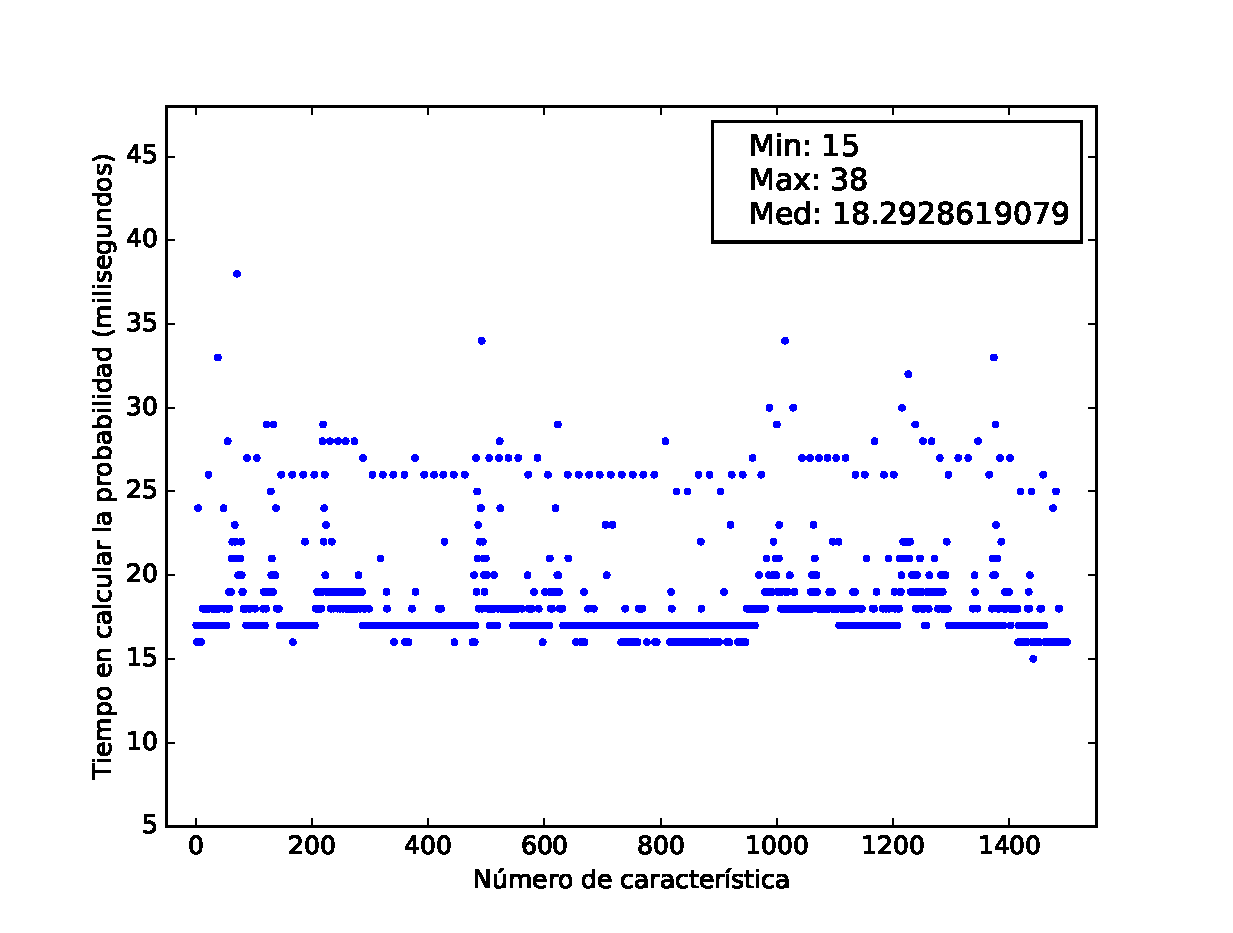
\includegraphics[width=0.8\hsize,angle=0]{plot_probs_times.eps}
        \linefigure
        \caption{Computing time analysis for a model consisting of 1500 features.}\label{fig:plot:probs:times}
\end{figure}

Figure~\ref{fig:plot:probs:times} shows the computing time required to calculate the probability of having
each feature in a product.
%In this case, the total time to obtain the probability for all the features is linear with respect to the total length of the analyzed term
%\mncomment{Que quiere decir esto? Suena raro porque yo esperaria complejidad $O(2^n)$ siendo $n$ el numero de probabilidades que salen en el termino. Pero vamos, que yo no  se mucho de complejidad!}\ccomen{Es cierto, no lo demostramos ni lo analizamos}.
%\acomen{Yo simplemente quitaría esa frase, lo de que la complejidad es lineal}
It is important to remark that there is a small variation in the processing time for calculating the probability of each single feature. We think that this variation is mainly caused by the inherent noise of the node where the experiment is launched (e.g. disk latencies, operating
system overhead, memory paging, etc.) and, therefore, it is not related to the algorithm itself.

Since the processing time for each feature is relatively low, being around milliseconds, a single delay in
the process scheduling may have a direct impact in the overall algorithm performance. Hence, this overhead
can be considered insignificant since, in general, the time for processing each feature in the model ranges
from 15 to 28 milliseconds.

The model used in the experiments has been executed several times, providing similar results. That is, the
major part of the features require between 15 and 20 milliseconds to be processed, while there is a small
portion of them requiring a processing time between 20 and 38 milliseconds.

\begin{figure}[h]
        \centering
        \linefigure
        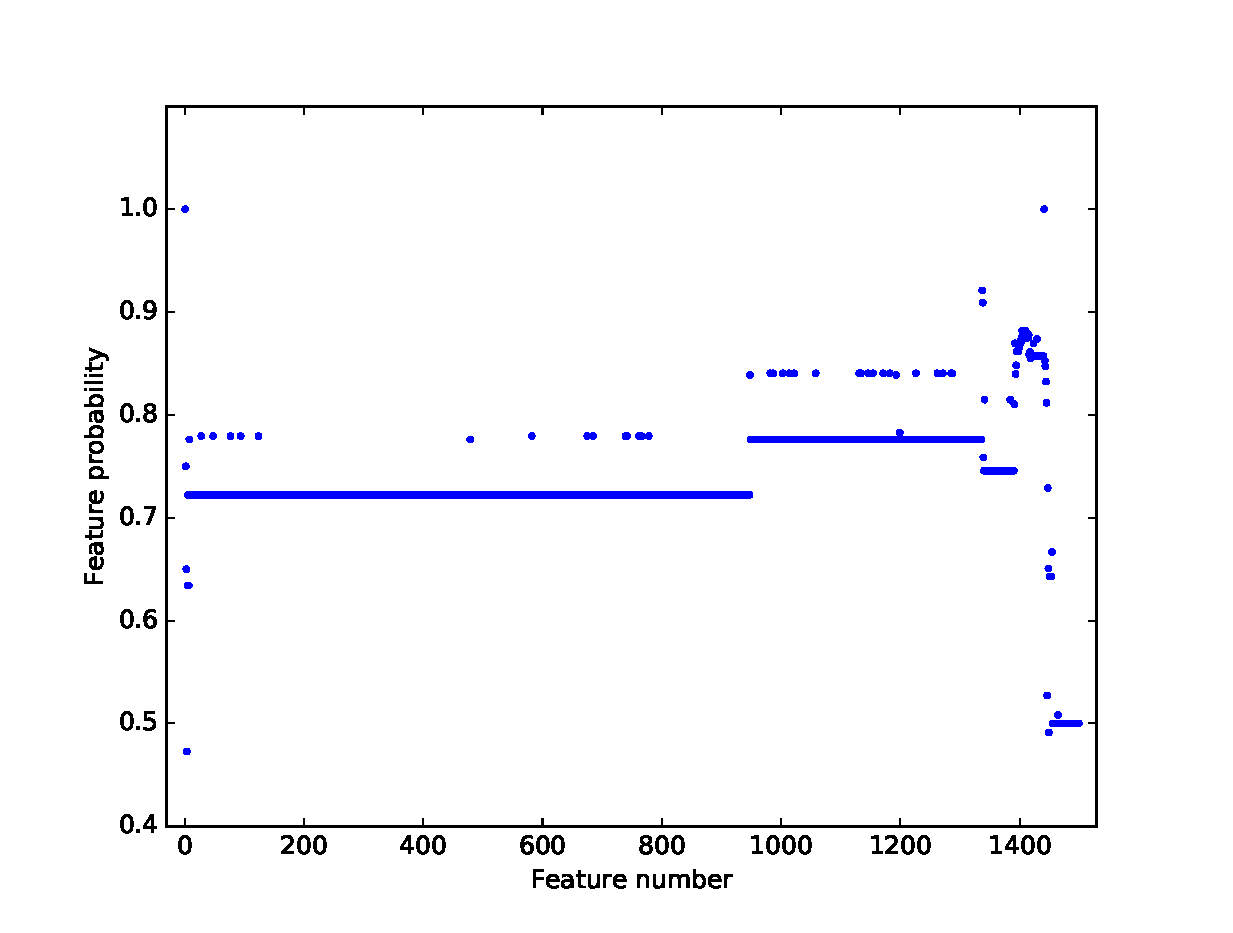
\includegraphics[width=0.8\hsize,angle=0]{plot_probs_probs.eps}
        \linefigure
        \caption{Probabilistic analysis for a 1500 features model.}\label{fig:plot:probs:probs}
\end{figure}

Figure~\ref{fig:plot:probs:probs} shows the probability of each feature in the analyzed model, where the $x$-axis
represents the feature ID and the $y$-axis represents the probability. For the sake of clarity, we provide a chart by sorting the features using its probability as sorting criteria (see Figure~\ref{fig:plot:probs:probs:sorted}).
This chart clearly shows that there exist different groups of features having a similar probability.
%
In this case, there are 450 features with, at least, a probability equal to 0.75 of being in a final product. As a conclusion,
this analysis might allow us to establish that by testing only the 28\% of the software product line components, we can ensure that
%the features
%included in,
at least, the 75\% of the generated products, are tested.

\begin{figure}[h]
        \centering
        \linefigure
        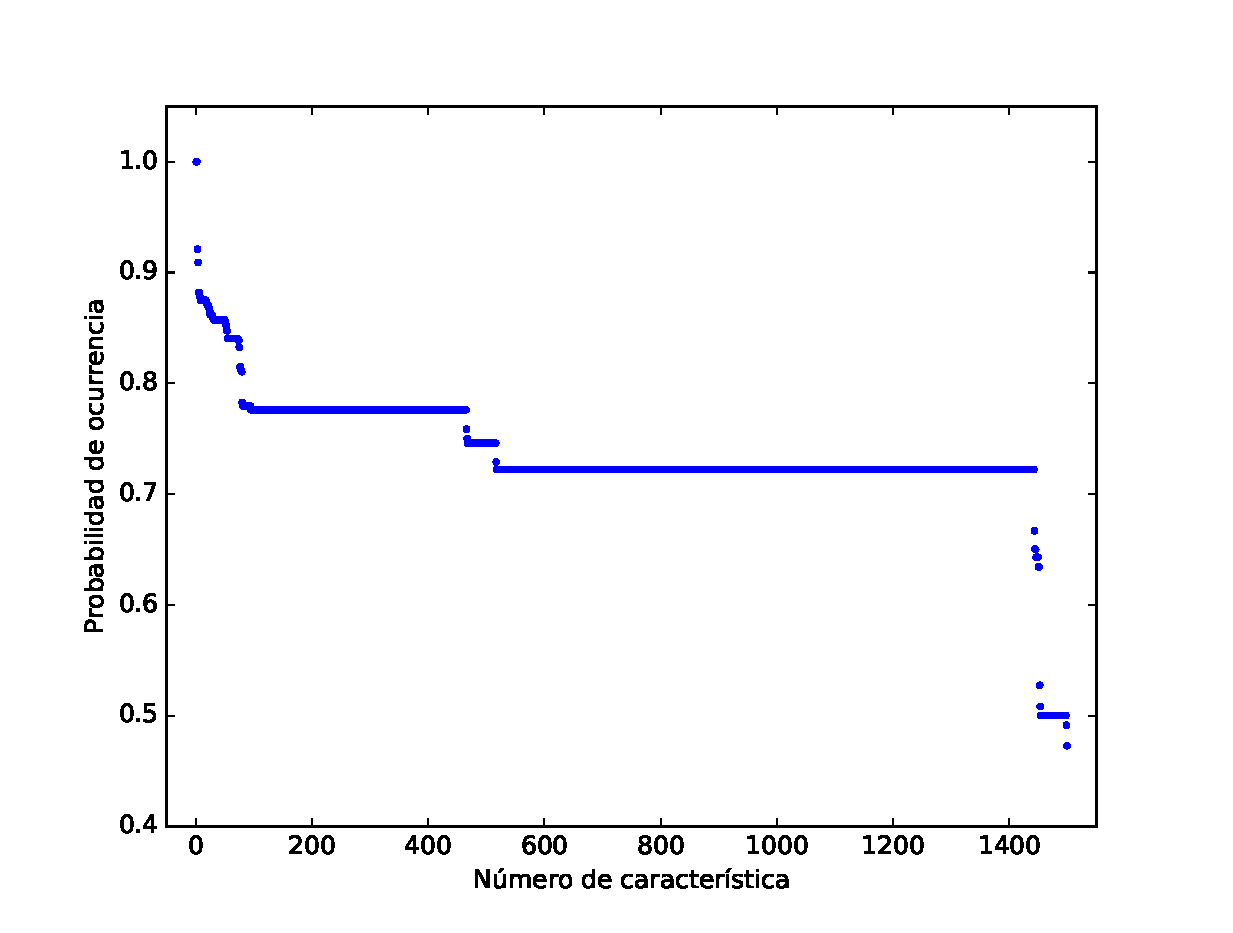
\includegraphics[width=0.8\hsize,angle=0]{plot_probs_probs_sorted.eps}
        \linefigure
        \caption{Probabilistic analysis for a 1500 features model, decreasingly sorted.}\label{fig:plot:probs:probs:sorted}
\end{figure}

%\begin{figure}[t]
%$$
%\begin{array}{ccc}
%\mathtt{Test}&\mathtt{Features}& \mathtt{Time}\\
%\#1& \feature{A},\feature{B} & 10\ units\\
%\#2& \feature{C},\feature{D} & 15\ units\\
%\#3& \feature{A},\feature{C},\feature{D} & 8\ units\\
%\#4& \feature{C},\feature{B} & 9\ units\\
%\end{array}
%$$
%\caption{Input parameter: test suite\label{fig:input:parameter}}
%\end{figure}

%We have two open issues:
%\begin{description}
%\item[Unit testing]  Let $P$ be a software product line, and $T_{unit}$ be a
%  test suite. Each test checks the correctness of a feature (i.e, %\feature{A} or \feature{B}).
%  We can compute the \emph{probability} of a feature. We test before those features with bigger probability.
%  \begin{itemize}
%  \item We can calculate the most frequent set of features in $P$ to test.
  %\item  We can provide a coverage of the test suite taking into account the percentage of appearance of each feature.
  %\end{itemize}

%\item[Integration testing] We have a test suite $T_{integration}$ where each test checks
%  the integration of a product.
%  Let us note that the integration of the product $\{\feature{A},\feature{B}\}$  can be different than
%  the integration of $\{\feature{A}, \feature{B},\feature{C}\}$.
%  \begin{itemize}
%  \item Which tests of the suite can be applied in this SPL?
 % \item What is the coverage of each test suite?
 % \end{itemize}


%\end{description}


%Next step is to associate to each integration test the time that
%it needs to be completed.
%For instance in Figure~\ref{fig:input:parameter} we represent some integration tests and the
%time that they need to be completed.



%\begin{quote}
%\emph{Let us consider an integration test suite and a probabilistic SPL $P$.
%If we only have $n$ time units, which is the \emph{best set} of tests
%to check the correctness of $P$? We say that a test is better than another
%test if its representativity (the probability to perform these features together) is higher.}
%\end{quote}

%\bprop
%        The previous problem is NP-hard\ccomen{I propose the transformation into the Subset Sum problem.}.
%\eprop

%Next we define the subset sum problem.

%\bdfn
%    Let $A = \{a_1, a_2, \ldots, a_n\}$ be a  set of natural numbers and $s$ be  a positive integer.
%    The subset sum problem checks if there is a subset $A'\subseteq A$ such that:  $$\sum_{a\in A'} = s$$
%\edfn

%In our previous problem we have a set of pairs $B=\{(p_{1},t_{1}),(p_{2},t_{2}),\ldots,(p_{n},t_{n})\}$ where
%$p_{i}$ is the probability to perform the test $i$ and $t_{i}$ is the time needed to perform this test, and
%two constants $P$ and $T$. $P$ will represent a probability value and $T$ a time value.
%We are looking for those pairs $(p_{i},t_{i}),\ldots,(p_{j},t_{j})\in B$ that
%$$
%\begin{array}{ll}
%p_{i}+\ldots +p_{j} &\geq P\\
%t_{i}+\ldots +t_{j} &\leq T\\
%\end{array}
%$$

%Let us consider that $p_{i}=t_{i}={a_i}$ and $P=T=s$.
%We can rewrite the previous problem into

%$$
%\left.
%\begin{array}{ll}
%a_{i}+\ldots +a_{j} &\geq s\\
%a_{i}+\ldots +a_{j} &\leq s\\
%\end{array}
%\right\}=
%a_{i}+\ldots +a_{j} = s\
%$$

%And we have the subset sum problem\ccomen{Please check because $p_{i}$ and $t_{i}$ can be reals while $s_{i}$ are integers}.


%\begin{enumerate}
%        \item We can create a GA to solve this problem.
%        \item We have that this problem is FPTAS~\cite{Ibarra:1975:FAA:321906.321909}.
%\end{enumerate}



%In order to obtain a set of tests that holds the previous issues, we propose
%two implementations.
%The first one is using a dynamic algorithm while the second one to use a genetic algorithm.

%\subsection{Dynamic algorithm}

% We adapted the dynamic algorithm of 0-1 Knapsack problem
%to our problem and we implemented it in python.


%We define a matrix $A$, where $A(i,j)$ contains the
%maximum value that can be attained from considering
%only the sum of the first i tests' probability that need at most j time units.


%$$
%A(i,j)=
%\left\{
%        \begin{array}{lll}
%        0 &\hspace*{3em}&\si i=0 \lor j = 0\\
%        A(i-1,j) & & \si t_i>j\\
%        \max{(A(i-1,j),p_{i}+A(i-1,j-t_i))} &&\si t_i \leq j
%        \end{array}
%\right.
%$$

%In our case, we will say that $A(n,T)$ is the solution if the sum of the  percentages
%of all elements involved in this solution is bigger than or equal to $P$. Otherwise we do not have a solution.


%For instance, in Table~\ref{figure:input:parameters} there are presented a set of 24
%different tests with their time consuming and its probability.
%For instance the first element, t1,9,150, means the test t1 needs 9 time units to be completed
%and the value associated with this test is 150\footnote{We could put here a measure, the probability or anything}.

%\begin{table}
%\centering

%\selectfont
%{\tt
%\begin{tabular}{|l|l|l|}
%\hline
%\#1,9,150 &
%\#2,13,35&
%\#3,153,200\\
%\#4,50,160&
%\#5,15,60&
%\#6,68,45\\
%\#7,27,60&
%\#8,39,40&
%\#9,23,30\\
%\#10,52,10&
%\#11,11,70&
%\#12,32,30\\
%\#13,24,15&
%\#14,48,10&
%\#15,73,40\\
%\#16,42,70&
%\#17,43,75&
%\#18,22,80\\
%\#19,7,20&
%\#20,18,12&
%\#21,4,50\\
%\#22,30,10&
%\#23,90,1&
%\#24,200,150\\
%\hline
%\end{tabular}}
%\caption{Input parameter (test,time,value) for the test selection algorithm.\label{figure:input:parameters}}
%\end{table}

% \begin{figure}[t]
% \centering
% includegraphics[scale=1]{GA_Flowchart_4}
% \caption{Scheme of GA.\label{scheme:genetic:algorithm}}
% \end{figure}





% After executing the dynamic algorithm, with the following input parameters a)
% the data presented in Table~\ref{figure:input:parameters} and T (the maximum time value) equals to 500,
% we obtain that {\tt \#1, \#2, \#3, \#4, \#5,
% \#7, \#8, \#9, \#11, \#12, \#16, \#17,
% \#18, \#19} and {\tt \#21}       conforms the final solution, and P =  1130.


% \subsection{Genetic Algorithm}

% Next we perform a genetic algorithm to discover a better solution.
% The GA structure is in Figure~\ref{scheme:genetic:algorithm}.
% With this algorithm we obtain values bigger than 1130.






% \subsubsection{Representation}
% We represent the possible solutions (those tests that hold the conditions) as follows:
% \begin{itemize}
%         \item Genotype: Given $n$ tests, we represent a solution with a binary (1/0) string
% of length $n$ where the position i determines whether the ith-test is included or not.
% The genotype space is complete, that is, any valid solution can be mapped in this array.
%         \item Phenotype: There are only some genotypes that are \emph{correct}. These are
% those that taking the $n'$, with $n'\leq n$ first $1$ bits from left to right of a genotype, we have that the sum of
% the time values associated with these tests is lower than or equal to T,
% and that the representativity of these tests is $\geq P$.
% \end{itemize}


% \subsubsection{Initial Population}
% We execute the algorithm with the parameters presented in Figure~\ref{fig:parameters:initial:population} in order to show
% how many initial population do we need.
% There is an interesting effect that this experiment reveals.
% The first and second graphs indicate that for populations smaller than 50 the chance for premature convergence seems to be rather high.
% Therefore we will consider that a good candidate for initial population is 500.

% \begin{figure}[t]
% \centering

% \begin{minipage}{0.45\hsize}\centering
%         \textbf{x}=10

% \includegraphics[scale=0.3]{graphs_basea/basea_diff_raw}
% \end{minipage}
% \begin{minipage}{0.4\hsize}\centering

%         \textbf{x}=50
% \includegraphics[scale=0.3]{graphs_baseb/baseb_diff_raw}

% \end{minipage}


% \begin{minipage}{0.45\hsize}\centering
%         \textbf{x}=200

% \includegraphics[scale=0.3]{graphs_based/based_diff_raw}
% \end{minipage}
% \begin{minipage}{0.4\hsize}\centering

%         \textbf{x}=500
% \includegraphics[scale=0.3]{graphs_basec/basec_diff_raw}

% \end{minipage}

% {\centering
% %\fontsize{7}{9}
% %\selectfont

% \begin{tabular}{|l|l|}
% \hline
% Representation  &Binary strings of length n\\
% Recombination   &One point crossover\\
% Recombination probability &     80\\
% Mutation        & Swap Mutator \\
% Mutation probability    & 2\% \\
% Parent selection        & Roulette\\
% Survivor selection      & Generational\\
% Population size         & \textbf{x} \\
% Termination condition   & Terminate the evolution based on the fitness stats\\
% Generations     & 100 \\
% \hline
% \end{tabular}}

% \caption{Comparing initial population\label{fig:parameters:initial:population}.}
% \end{figure}



% \subsubsection{Recombination probability}
% Next we study the effect of changing the recombination probability.
% In Figure~\ref{fig:parameters:recombination} we show the max fitness, average fitness and
% minimum fitness of the population, in each generation, using the probability values 0.1, 0.4, 0.8 and 1 for recombination.
% We will use 0.8 in the rest of experiments because a) we obtain the maximum fitness, and b) the difference between maximum and minimum is low.

% Let us also note that adding more values of recombination probability (i.e, 100\%), that is also presented in
%  Figure~\ref{fig:parameters:recombination} does not imply to have better fitness solutions. So, this value should be high
% but not 100\%.

% \begin{figure}[t]

% \centering

% \begin{minipage}{0.5\hsize}\centering
%         \textbf{x}=0.1

% \includegraphics[scale=0.3]{graphs_basee/basee_maxmin_fitness}
% \end{minipage}
% \begin{minipage}{0.4\hsize}\centering

%         \textbf{x}=0.4
% \includegraphics[scale=0.3]{graphs_basef/basef_maxmin_fitness}

% \end{minipage}


% \begin{minipage}{0.50\hsize}\centering
%         \textbf{x}=0.8

% \includegraphics[scale=0.3]{graphs_baseg/baseg_maxmin_fitness}
% \end{minipage}
% \begin{minipage}{0.4\hsize}\centering

%         \textbf{x}=1
% \includegraphics[scale=0.3]{graphs_baseh/baseh_maxmin_fitness}

% \end{minipage}


% {\centering
% %\fontsize{7}{9}
% %\selectfont

% \begin{tabular}{|l|l|}
% \hline
% Representation  &Binary strings of length n\\
% Recombination   &One point crossover\\
% Recombination probability &     \textbf{x}\\
% Mutation        & Swap Mutator \\
% Mutation probability    & 2\% \\
% Parent selection        & Roulette\\
% Survivor selection      & Generational\\
% Population size         & 500 \\
% Termination condition   & Terminate the evolution based on the fitness stats\\
% Generations     & 100 \\
% \hline
% \end{tabular}}

% \caption{Comparing recombination probability\label{fig:parameters:recombination}.}
% \end{figure}

% \subsubsection{Mutation operator}

% We define two mutation operators in the chromosomes. The first one: swap means to change
% the element i with the element j. The second one: Integer range, means that we change a bit
% randomly.

% In our algorithm we are able to use both mutators operators.
% In Figure~\ref{fig:parameters:mutation:operator} the effects of executing swap, integer range or both
% are presented.

% We can observe that only swap let the fitness score to be regular with respect to the number of generations.
% When we change randomly a bit in the chromosomes then the fitness score cannot be predictable.

% \begin{figure}[t]

% \centering

% \begin{minipage}{0.5\hsize}\centering
%         \textbf{x}=Swap

% \includegraphics[scale=0.3]{graphs_basei/basei_maxmin_fitness}
% \end{minipage}
% \begin{minipage}{0.45\hsize}\centering

%         \textbf{x}=Swap and Integer Range

% \includegraphics[scale=0.3]{graphs_basej/basej_maxmin_fitness}

% \end{minipage}

% \begin{minipage}{0.5\hsize}\centering
%         \textbf{x}=Integer Range

% \includegraphics[scale=0.3]{graphs_basek/basek_maxmin_fitness}
% \end{minipage}
% %\begin{minipage}{0.45\hsize}\centering

% {\centering

% %\fontsize{7}{9}
% %\selectfont
% \begin{tabular}{|l|l|}
% \hline
% Representation  &Binary strings of length n\\
% Recombination   &One point crossover\\
% Recombination probability &     0.8\\
% Mutation        & \textbf{x} \\
% Mutation probability    & 2\% \\
% Parent selection        & Roulette\\
% Survivor selection      & Generational\\
% Population size         & 500 \\
% Termination condition   & Terminate the evolution based on the fitness stats\\
% Generations     & 100 \\
% \hline
% \end{tabular}}
% %\end{minipage}

% \caption{Comparing Mutation Operators\label{fig:parameters:mutation:operator}.}
% \end{figure}

% \subsubsection{Parent Selection}

% Finally we compare the parent selection methodology used in our algorithm.
% We implement three kind of selections: Rank, Roulette and Tournament.
% In our experiments we decided to use Roulette because it is always increasing,
% and it seems that we can continue improving the valuation of the set of tests over time.
% Moreover the others seem to be saturated.
% \begin{figure}[t]

% \centering

% \begin{minipage}{0.5\hsize}\centering
%         \textbf{x}=Rank

% \includegraphics[scale=0.3]{graphs_baser/baser_maxmin_fitness}
% \end{minipage}
% \begin{minipage}{0.4\hsize}\centering

%         \textbf{x}=Roulette
% \includegraphics[scale=0.3]{graphs_bases/bases_maxmin_fitness}

% \end{minipage}

% \begin{minipage}{0.50\hsize}\centering
%         \textbf{x}=Tournament

% \includegraphics[scale=0.3]{graphs_baset/baset_maxmin_fitness}
% \end{minipage}

% %\begin{minipage}{0.45\hsize}\centering


% {\centering
% %\fontsize{7}{9}
% %\selectfont
% \begin{tabular}{|l|l|}
% \hline
% Representation  &Binary strings of length n\\
% Recombination   &One point crossover\\
% Recombination probability &     0.8\\
% Mutation        & Swap \\
% Mutation probability    & 2\% \\
% Parent selection        & \textbf{x}\\
% Survivor selection      & Generational\\
% Population size         & 500 \\
% Termination condition   & Terminate the evolution based on the fitness stats\\
% Generations     & 100 \\
% \hline
% \end{tabular}}
% %\end{minipage}

% \caption{Comparing parent selection\label{fig:parameters:parent:selection}.}
% \end{figure}

%%% Local Variables:
%%% mode: latex
%%% TeX-master: "main"
%%% End:


\section{Conclusions}
\label{section:jstat:concs}

Once described all the problems related to the combinatory explosion
for some of the algebra's operators, we aim to generate enough information
allowing to determine the probability of a probability in the valid
products set.
%
To do so we have defined new syntactical operators for the probabilistic
extension. Once defined, we have represented the extension to give a logical
meaning to these semantic rules based on the operational semantics
and denotational semantics.
%
Also this extension was proven to be consistent against the presented definitions
and with the non probabilistic models.
%
The implementation of this extension allows to compute and calculate the probability of the features among the valid products.

%%% Local Variables: 
%%% mode: latex
%%% TeX-master: "main"
%%% End: 




\bibliographystyle{elsarticle-num}
\bibliography{concu,concuPL}

%\bibliographystyle{abbrv}

\end{document}

%%% Local Variables:
%%% mode: latex
%%% TeX-master: t
%%% End:
